\documentclass[a4paper,12pt,twoside]{article}
        \usepackage{graphicx,type1cm,eso-pic,color}
        \usepackage{hyperref}
        \usepackage{longtable}
        \usepackage{amsmath,amssymb} 
        \usepackage[latin1]{inputenc}
        \usepackage[OT1]{fontenc}
        \usepackage{setspace}
        \usepackage{epigraph}



\hypersetup{
     backref=true,    %permet d'ajouter des liens dans...
     pagebackref=true,%...les bibliographies
     hyperindex=true, %...les index.
     colorlinks=true, %colorise les liens
     breaklinks=true, %permet le retour à la ligne dans les liens trop longs
     urlcolor= blue, %couleur des hyperliens
     linkcolor= black, %couleur des liens internes
     bookmarks=true, %créé des signets pour Acrobat
     bookmarksopen=true,            %si les signets Acrobat sont créés,
                                    %les afficher complètement.
     pdftitle={Hadronization Analysis Note (EG2)}, %informations apparaissant dans
     pdfauthor={Raphael Dupre},     %dans les informations du document
     pdfsubject={Physics}          %sous Acrobat.
}

\setlength{\hoffset}{-18pt}  	
\setlength{\oddsidemargin}{20pt} 	% Marge gauche sur pages impaires
\setlength{\evensidemargin}{20pt} 	% Marge gauche sur pages paires
\setlength{\marginparwidth}{54pt} 	% Largeur de note dans la marge
\setlength{\textwidth}{440pt} 		% Largeur de la zone de texte (17cm)
\setlength{\voffset}{18pt}	        % Bon pour DOS
\setlength{\marginparsep}{7pt} 	 	% Séparation de la marge
\setlength{\topmargin}{0pt} 	        % Pas de marge en haut
\setlength{\headheight}{13pt} 		% Haut de page
\setlength{\headsep}{0pt}              % Entre le haut de page et le texte
\setlength{\footskip}{27pt} 	        % Bas de page + séparation
\setlength{\textheight}{600pt} 	 	% Hauteur de la zone de texte (25cm)


\newcommand{\xbp}{$x_{Bj}$}
\newcommand{\xb}{$x_{Bj}~$}
\newcommand{\ptp}{$p_\perp^2$}
\newcommand{\pt}{$p_\perp^2~$}
\newcommand{\dptp}{$\Delta \langle p_\perp^2 \rangle$}
\newcommand{\dpt}{$\Delta \langle p_\perp^2 \rangle ~$}


\makeatother

\title{Study of the hadronization of $\pi^-$}

\author{Rapha\"el \textsc{Dupr\'e}, 
Lamiaa \textsc{El Fassi}\thanks{also {\it Rutgers University}} , 
Kawtar \textsc{Hafidi} ... \\ 
{\it Physics Division, Argonne National Laboratory,} \\
{\it Argonne, Illinois 60439, USA} }

\date{\today}

\begin{document}

\maketitle

%doublespacing
%onehalfspacing
%\linenumbers
\renewcommand{\baselinestretch}{1.10}

\begin{abstract}
Hadronization is the process by which energetic quarks transform into 
colorless hadrons. The process is non-perturbative, therefore, only 
qualitative understanding can be achieved, and using phenomenological models 
is necessary. It is believed that hadronization has two distinct phases: 
the quark propagation phase, where the quark emit gluons until it neutralizes 
its color by forming a pre-hadron and the hadron formation phase, where the 
pre-hadron evolves into a hadron. Those process are respectively characterized 
by the production time and the formation time. By comparing hadron production 
on different nuclei, one can measure variables with different sensitivities 
to the hadronization phases, the two principal variables are: the transverse 
momentum broadening, that is believed to be tightly connected to quark energy 
loss and the multiplicity ratio, which is a measure of the hadron attenuation 
in the medium.

The goals of the experiment E-02-104 are to study both quark propagation
and hadronization dynamic using various nuclear target.
In this analysis we focus on two particles, the negative pion and the proton.
Our goals are to constrain the theoritical models and extract the production
time using precise multidimensional analysis of $\pi^+$ and $\pi^-$ to enlight possible
new physical processes with a precise analysis of proton production in nuclei.

\end{abstract}

\newpage

\tableofcontents

\newpage


\section{Introduction}
\label{physics}

The hadronization process by which partons fragment into hadrons is 
experimentally well studied, and the associated fragmentation functions are extracted from the fit of experimental data over a wide range of kinematics~\cite{Albino:2008fy}. Nevertheless, the hadron formation is a non perturbative process, which can not be described theoretically, but only via a systematic study of the whole hadronization mechanism (see figure \ref{fig:hadro}) for energies above the resonance region. In Deep Inelastic Scattering (DIS), the virtual photon interacts with a quark which propagates quasi-free emitting gluons during the so-called production time. After neutralizing its color, the quark becomes a pre-hadron that eventually evolves to a full hadron after the formation time. The advantage of using nuclear targets is that the hadronization process occurs, at least partially, inside the nuclear matter, which allows the extraction of hadronization time-scales by comparing different behavior of quarks and colorless pre-hadrons in the medium. The measurement of pions production is especially suited for this analysis because they are easy to detect and abundant in the nuclear deep inelastic scattering (nDIS).

\begin{figure}[htbp]
\centering
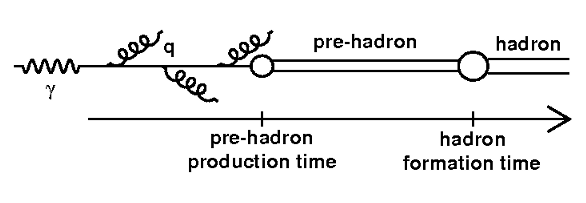
\includegraphics[width=10cm] {fig/hadro.png} 
\caption {Sketch of the hadronization process.}
\label{fig:hadro}
\end{figure}

The hadronization in nuclear matter is also a key process for the study of the Quantum 
Chromo-Dynamics theory (QCD) because it leads to major theoretical 
uncertainties in numerous measurements. DIS experiments at JLab energies are 
well suited to test different theoretical models of hadronization, including 
the ones used for Relativistic Heavy Ion Collisions (RHIC). The main advantage 
of testing models in lepton scattering is that the size of cold nuclei is 
stable and known, while in RHIC the nuclear medium is hot and evolving 
introducing many parameters and unknowns. The hadronization process can also 
give important information about nuclei through the quark energy loss, for example, Arleo's model~\cite{Arleo:2003yf} correlates the quark energy loss with a gluon density, and Kopeliovich et al.'s model~\cite{Kopeliovich:2010aa} correlates the $\Delta \langle P_T^2 \rangle$ with the saturation scale. Other models \cite{Gallmeister:2007an} utilize different assumptions to describe the pre-hadron evolution into a full hadron. Therefore, high precision measurements are very important to discriminate between different models. 

A quantitative understanding of the hadronization process in nuclei is also of importance for neutrino experiments. Indeed, these use nuclear targets to maximize their cross sections and therefore have to account for the nuclear effects, including hadronization. 

In order to best constrain the models with our data, we extracted our results using tight multi-dimensional binning. That is possible because of the high statistics of our EG2 data, which allowed the study of both pion production on a wide kinematic range.

We present in section \ref{sec:theo} a highlight of different models' families describing the hadronization process in hot and cold nuclear matter, then in section \ref{sec:exp} we make a rapid overview of published results. For more detailed information, we refer the readers to the review of Accardi {\it et al.} \cite{Accardi:2009qv}.


\subsection{Kinematic Variables and Observables}

In this analysis, we use the following Semi-Inclusive Deep Inelastic Scattering (SIDIS) variables:
\begin{itemize}
 \item $\nu = E_i - E_f$ is the energy transferred by the lepton probe in the laboratory frame, where $E_i$ is the beam energy and $E_f$ is the scattered electron energy,
 \item $Q^2 = 4 E_i E_f \sin ^2(\theta_e / 2)$ is the 4-momentum transferred, where $\theta_e$ is the polar angle of a scattered electron,
 \item $x_{Bj} = {{Q^2} \over {2 M_n \nu}}$ is the proton momentum fraction carried by the struck quark, with $M_n$ the nucleon mass,
 \item $W^2 = M_n^2 - Q^2 + 2 M_n \nu$ is the mass squared of the hadronic final state,
 \item $z_h = E_h / \nu$ is the virtual photon energy fraction carried by the measured hadron, with $E_h$ the hadron energy,
 \item $P_T^2$ is the hadron transverse momentum measured with regard to the virtual photon direction,
 \item $\phi_h$ is the angle between the leptonic plane (containing initial and scattered electrons) and the hadronic plane (containing the virtual photon and a measured hadron),
 \item $x_F = P_L/P_L^{max}$ is the longitudinal momentum fraction carried by the hadron, and calculated with respect to the virtual photon direction in the laboratory frame.
 Effectively this translate into: $$ x_F = 2 {z M_n \nu^2 - z Q^2 \nu - (M_n+\nu)(\boldsymbol{P_h \cdotp q}) \over (W^2-M_h^2) \sqrt{\nu^2+Q^2} } .$$
\end{itemize}
%TODO Add t

We define the multiplicity ratio as:
\begin{equation}
R_A^h (Q^2,\nu,z_h,P_T^2) = {{N_A^h (Q^2,\nu,z_h,P_T^2) / N_A^e (Q^2,\nu)} 
                       \over {N_D^h (Q^2,\nu,z_h,P_T^2) / N_D^e (Q^2,\nu)}},
\end{equation}
$N^e_A$ and $N_A^h$ are the number of electrons and semi-inclusive hadrons $h$ measured simultaneously on a target $A$. The multiplicity ratio represents the relative production rate of the hadron $h$ in a nuclear target~$A$.
\newline

We define the transverse momentum broadening as:
\begin{equation}
\Delta \langle P_T^2 \rangle = \langle P_T^2 \rangle_A - \langle P_T^2 \rangle_D,
\end{equation}
where $\langle P_T^2 \rangle_A$ is the mean transverse momentum measured on a target $A$.


\subsection{Theoretical Efforts}
\label{sec:theo}

The different models explaining the data can be separated in three families;
some assume that the quark looses energy in the medium and that either the hadronization occurs outside the medium or the hadronic interaction is 
negligible, others neglect the quark energy loss and consider
only the hadron and pre-hadron absorption, and the third category considers both
interactions. For illustration, we will give an example of each case, but for more detailed information, we refer the readers again to the Accardi {\it et al.} review~\cite{Accardi:2009qv}, which is more exhaustive and highlights also models describing RHIC's experiments.

In \cite{Wang:2002ri}, E.~Wang and X.-N.~Wang, described HERMES data using only 
the parton energy loss, hence the observed suppression is due to the fact that a lower energy quark fragments into a low number of hadrons at a very low $z$. This kind of model is suitable for both RHIC and nDIS experiments since it permits a common interpretation of hadron suppression in the nuclear matter. Moreover, various calculations have described the parton energy loss in the nuclear medium using the $\hat q$ (GeV$^2$ fm$^{-1}$) parameter, that is defined as the quark transverse momentum normalized by its propagation path length. In these models, $\hat q$ can also be related to the $\Delta \langle P_T^2 \rangle$ observable. The main difficulty of quark energy loss models is the lack of a coherent description for both multiplicity ratios and $P_T$ broadening behaviors. Recent models used a $\hat q$ to reproduce multiplicity ratio, which is too large to describe the transverse momentum broadening.
% TODO Add a ref

The transport model, GiBUU~\cite{Gallmeister:2007an}, is based on the 
Boltzmann equation that employs hadronic and pre-hadronic interactions in the nuclear matter without involving any quark energy loss. This model reproduces very well most of hadrons' multiplicity ratios, however, it failed to describe the transverse momentum broadening. 
%$\Delta \langle P_T^2 \rangle$ variable is not described at all by 

Finally, B.Z.~Kopeliovich et al. \cite{Kopeliovich:2008uy} described the process by neither neglecting the quark energy loss nor the hadron absorption, but used both $\Delta \langle P_T^2 \rangle$ and $R_A^h$ observables to differentiate between these effects. In that case, the transverse momentum broadening is correlated with the quark energy loss, and the suppression of multiplicity ratios is explained by the hadron absorption in the nuclear medium.

To conclude it is important to point out that no consensus is reached on which 
mechanisms are dominant. It is, therefore, important to perform precise measurements with the appropriate observables to disentangle these effects.


\subsection{Previous Mesurements}
\label{sec:exp}

Hadron multiplicity ratios in nuclei were originaly measured in numerous lepton 
facilities: L.S.~Osborne {\it et al.} \cite{Osborne:1978ai} at SLAC,
L.~Hand {\it et al.} \cite{Hand:1978tx}, the E665 collaboration \cite{Adams:1994ri} at FNAL, and the European Muon Collaboration \cite{Arvidson:1984fz,Ashman:1991cx} at CERN. These measurements revealed the main features of the hadronization mechanism
in nuclei by showing a suppression of hadrons' production in heavy nuclei.
This suppression appears to be reduced at higher $\nu$ and lower $z$, at very 
low $z$ it can even change sign and become an increased yield. 

Figures \ref{fig:her1}, \ref{fig:her2} and \ref{fig:her3} show a sample of 
the most recent HERMES data~\cite{Airapetian:2007vu} from DESY, where numerous hadrons were individually studied, and new variables linked with the transverse momentum were used in addition to the traditional multiplicity ratio.

\begin{figure}[htbp]
\centering
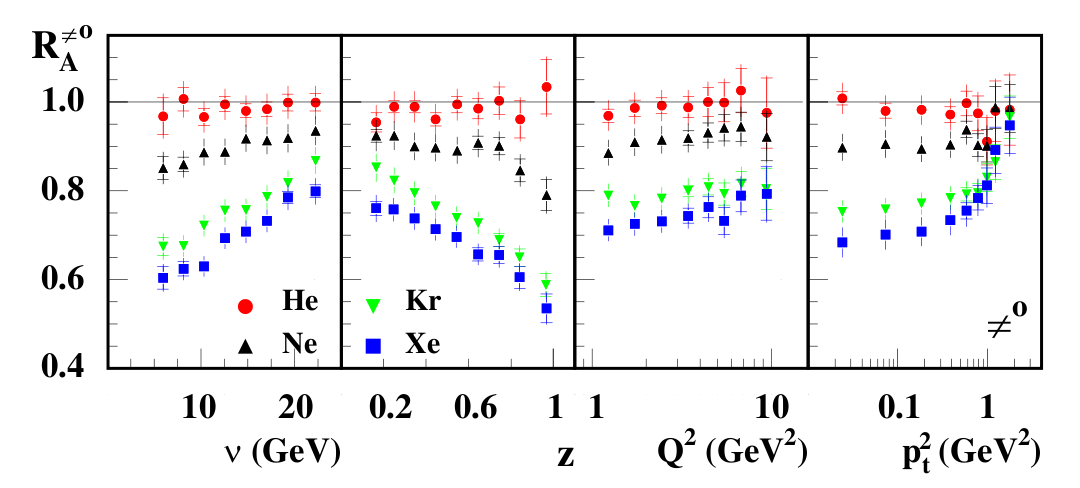
\includegraphics[width=14cm] {fig/Hermes/pi0hermes.png} 
\caption {Multiplicity ratios of $\pi^0$ as a function of various kinematical variables from the HERMES collaboration \cite{Airapetian:2003mi}}
\label{fig:her1}
\end{figure}

\begin{figure}[htbp]
\centering
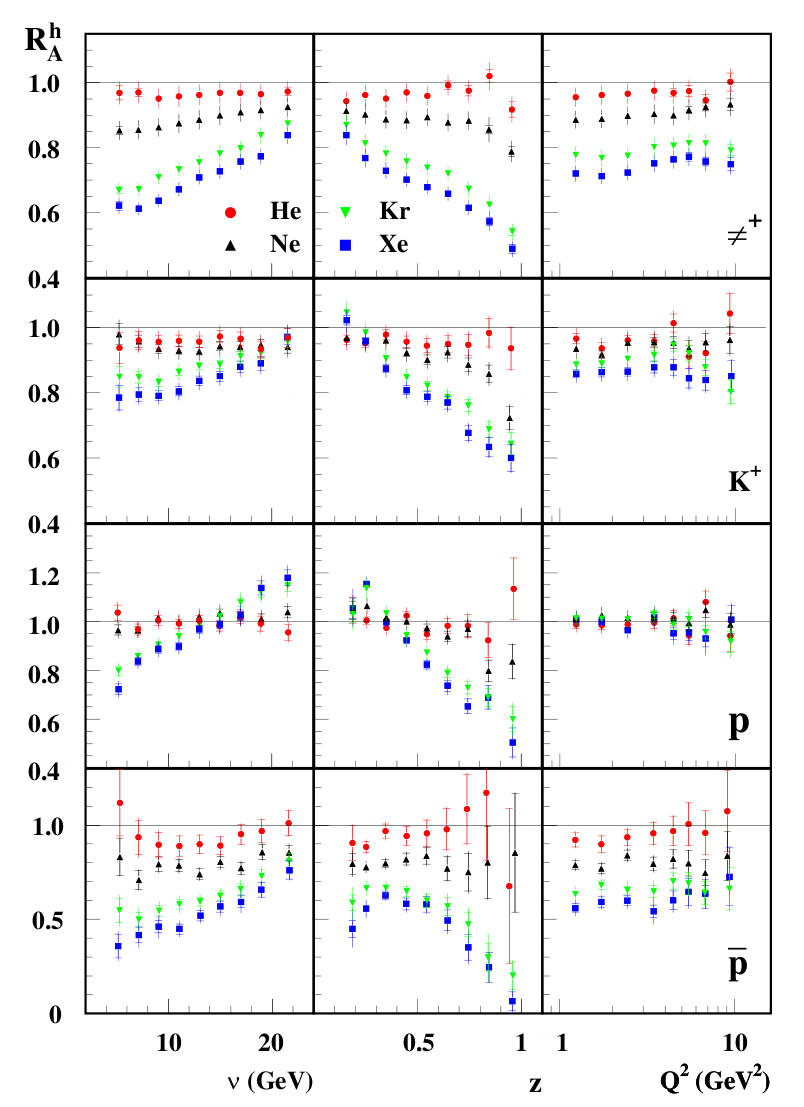
\includegraphics[width=14cm] {fig/Hermes/hermes1.png} 
\caption {Multiplicity ratios of $\pi^+$, K$^+$, protons and anti-protons as a 
function of various kinematical variables from the HERMES collaboration \cite{Airapetian:2007vu}}
\label{fig:her2}
\end{figure}

\begin{figure}[htbp]
\centering
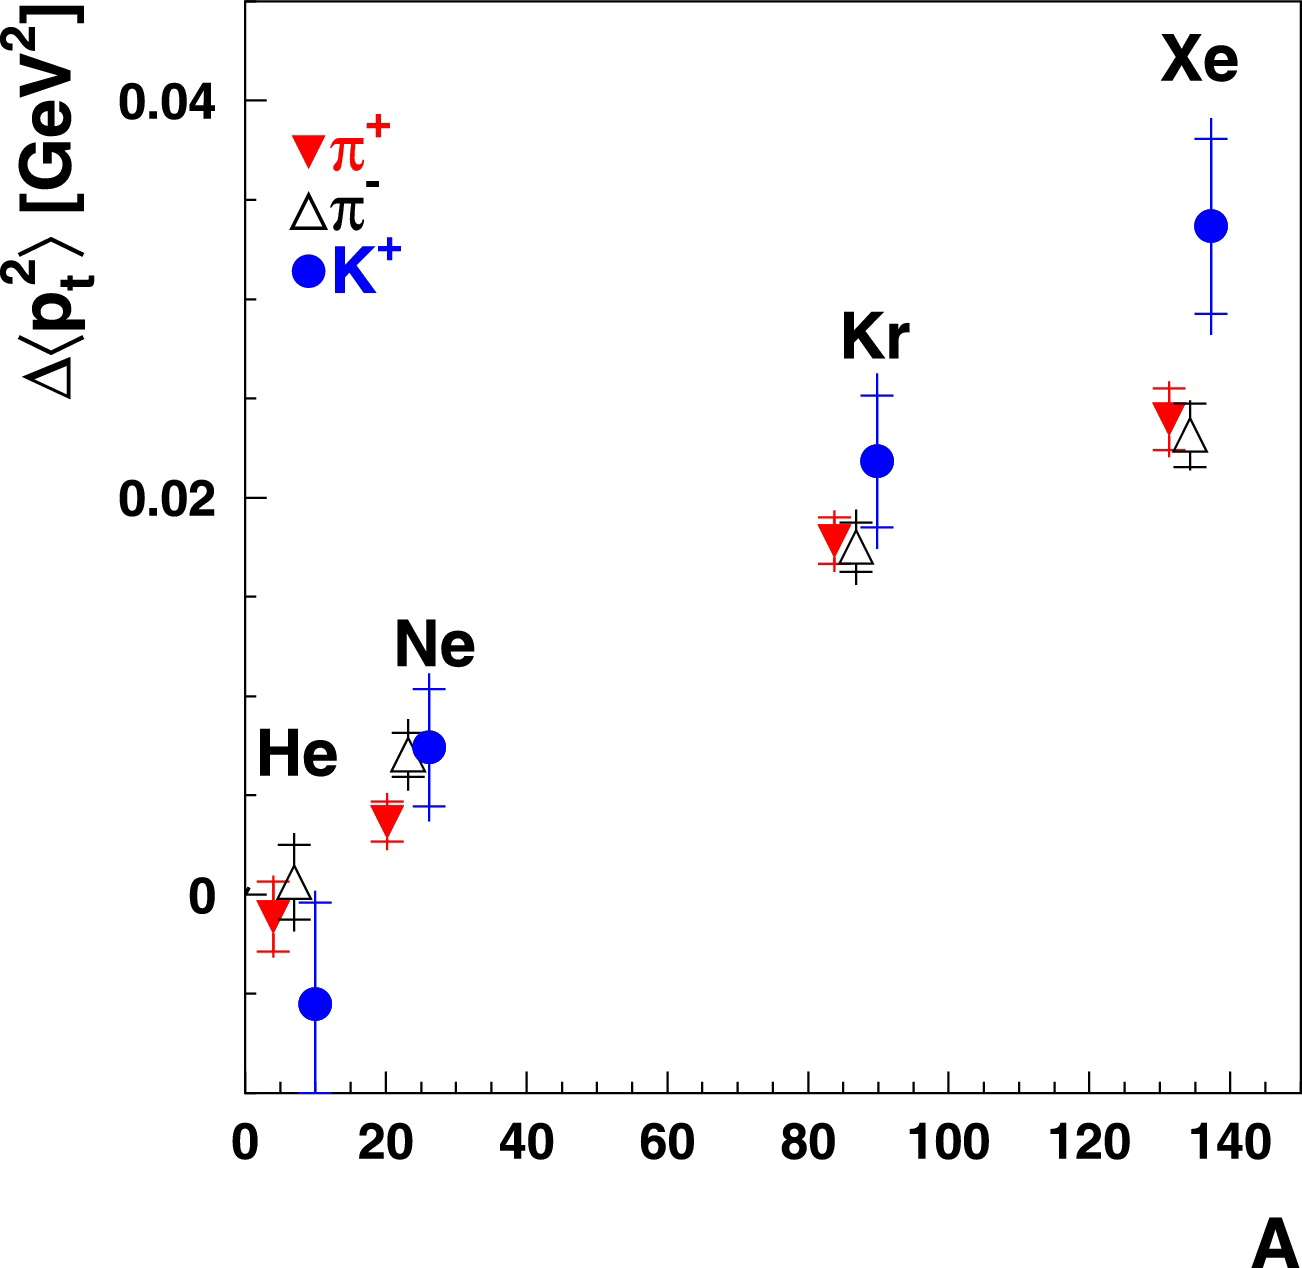
\includegraphics[width=7cm] {fig/Hermes/pthermes.png} 
\caption {Transverse momentum broadening for various particles from the HERMES collaboration \cite{Airapetian:2009jy}}
\label{fig:her3}
\end{figure}

The good precision of HERMES data shed light on new hadronization features, 
such as the behavior of K$^+$s, which have less attenuation than pions (see 
figure \ref{fig:her1}) but an excess in $\Delta \langle P_T^2 \rangle$. It is 
notable that it is difficult to reproduce this behavior in models where only 
one hadronization stage is taken into account to explain all effects. Likewise, 
the different behavior of protons compared to anti-protons (see figure 
\ref{fig:her2}) is interesting but most existing models do not treat baryon 
hadronization yet.



\section{Data Analysis}
\label{chap:analysis}

\subsection{Introduction}

This chapter treats of the analysis of the data taken in CLAS for the 
experiments E-02-104 \cite{Brooks:2002aa} and E-02-110 \cite{Hafidi:2002aa}.
The code name for the run is {\it eg2}, it was composed of three phases 
labeled {\it a}, {\it b} and {\it c}. The analysis is performed on the data 
collected in the beginning of 2004 during the third phase ({\it eg2c}), for 
which the beam energy was 5.014 GeV\footnote{The other phases gave a small 
amount of data at a beam energy of 4 GeV.}.

As the two experiments, running simultaneously, aimed at comparing deuterium 
with heavier nuclei, it was decided to use a double target system 
\cite{Hakobyan:2008zz}. The first target is filled with liquid deuterium and 
the second is a solid target. The latter can be made of carbon, aluminum, 
iron, tin or lead and changed remotely (the system is shown in figure 
\ref{fig:phototarget}). The two targets are separated by only 4~cm in order to reduce
the acceptance differences between them. The 
advantage to have the two targets in the beam line simultaneously
is that several systematic effects related to the beam 
and detector properties will cancel in the nuclear ratio.

\begin{figure}[htbp]
\centering
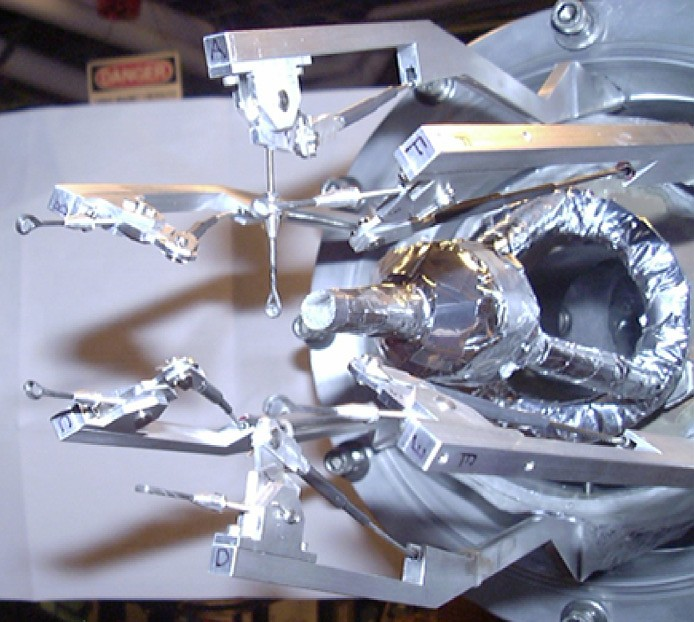
\includegraphics[width=7cm] {chap5-fig/PhTar.jpg} 
\caption {Picture of the target system of the {\it eg2} run. The cryogenic target is 
in the back, enveloped in aluminum foils. The solid targets are held by mechanical arms
allowing to change targets remotely, in the picture the top arm is in the beam line.}
\label{fig:phototarget}
\end{figure}

The analysis of the experiment E-02-110, focusing on the study of color 
transparency effects, has been approved recently \cite{ElFassi:2008}. As this 
analysis went through a careful review by the CLAS collaboration, we use
similar analysis methods when possible. In particular, the electron selection 
presented here is very similar to theirs; the main difference being a new 
target determination method.

In the section \ref{sec:pid}, we identify the following particles e$^-$, 
$\pi^-$ and $\pi^+$ using a series of cuts on the various 
detector outputs. For pions, we use the signal in the drift chambers (DC) and 
in the scintillator counters (SC), for which we require a positive status (global and DC) 
from the reconstruction code. For electron identification, we use signals from 
all detector parts DC, Cherenkov Counters (CC), SC and Electromagnetic 
Calorimeter (EC).

Once particles are identified, we can extract the observables (multiplicity 
ratio and transverse momentum broadening). The method is presented in the 
section \ref{sec:obs}, however these need several corrections presented in the 
section \ref{sec:corrections}. The 
two main corrections are the acceptance of the detector and the radiative 
effects, both are evaluated using Monte-Carlo generator. The evaluation of 
the systematic errors is presented in the section \ref{sec:TotSys}.
The analysis' final results are presented and discussed in the next chapter.

\subsection{Particle Identification}
\label{sec:pid}

\subsubsection{Electron Identification}

First, we apply a fiducial cut on the EC to remove the electrons detected on 
the edge of the calorimeter ($U_{EC}>40$~cm, $V_{EC}<360$~cm and 
$W_{EC}<395$~cm in the calorimeter's coordinates). These are problematic hits 
because the generated electromagnetic shower might be partly outside the 
detector, leading to a wrong measurement of the energy deposited.

To reject pions, we apply cuts on the energy deposited
in the EC using the measurements in the inner ($E_{in}$) and the 
outer part ($E_{out})$ of the calorimeter:

\begin{equation}
\label{einout}
\mu  \left[1-\frac{0.3}{\sqrt{a}}\right] - \frac{E_{in}}{p} \leq 
\frac{E_{out}}{p} \leq 
\mu  \left[1+\frac{0.3}{\sqrt{b}}\right] - \frac{E_{in}}{p},
\end{equation}

where $\mu = 0.271$ is the mean of the fraction of the energy deposited in the 
calorimeter by electrons, the $a$ parameter is set at 0.5 and the parameter 
$b$ is a function of momentum given in table \ref{tab:ecoutin-par}. The 
adjustment of $b$ is motivated by the non-linear dependence of the energy 
deposited as a function of the particle's momentum (see figure \ref{eleEC}). As pions are 
minimum ionizing particles, they are expected to lose a constant energy in 
the inner part of the calorimeter (around 30~MeV), regardless of their 
momentum. Therefore, by requesting more than 60~MeV to be deposited, we 
efficiently cut the pion contamination (see figure~\ref{eleECi}).

\begin{table}[tbp]
  \centering
  \begin{tabular}{@{} cc @{}}
    \hline
    Momentum bin (GeV/c)& Parameter b \\ 
    \hline
    0.5 - 0.7 & 0.85 \\
    0.7 - 0.9 & 0.8  \\
    0.9 - 1.1 & 0.85 \\
    1.1 - 1.3 & 1.05 \\
    1.3 - 1.5 & 1.1  \\
    1.5 - 1.7 & 1.35 \\
    1.7 - 1.9 & 1.35 \\
    1.9 - 2.1 & 1.45 \\
    2.1 - 2.3 & 1.35 \\
    2.3 - 2.5 & 1.35 \\
    2.5 - 2.7 & 1.35 \\
    2.7 - 2.9 & 1.3  \\
    2.9 - 3.1 & 1.35 \\
    3.1 - 3.3 & 1.35 \\
    3.3 - 3.5 & 1.5  \\
    3.5 - 3.7 & 1.6  \\
    3.7 - 3.9 & 1.8  \\
    3.9 - 4.1 & 1.8  \\
    4.1 - 4.3 & 1.8  \\
    4.3 - 4.5 & 1.8  \\
    \hline
  \end{tabular}
  \caption{Values of the parameter $b$ used in equation \ref{einout} for 
           different momentum ranges.}
  \label{tab:ecoutin-par}
\end{table}

\begin{figure}[p]
\centering
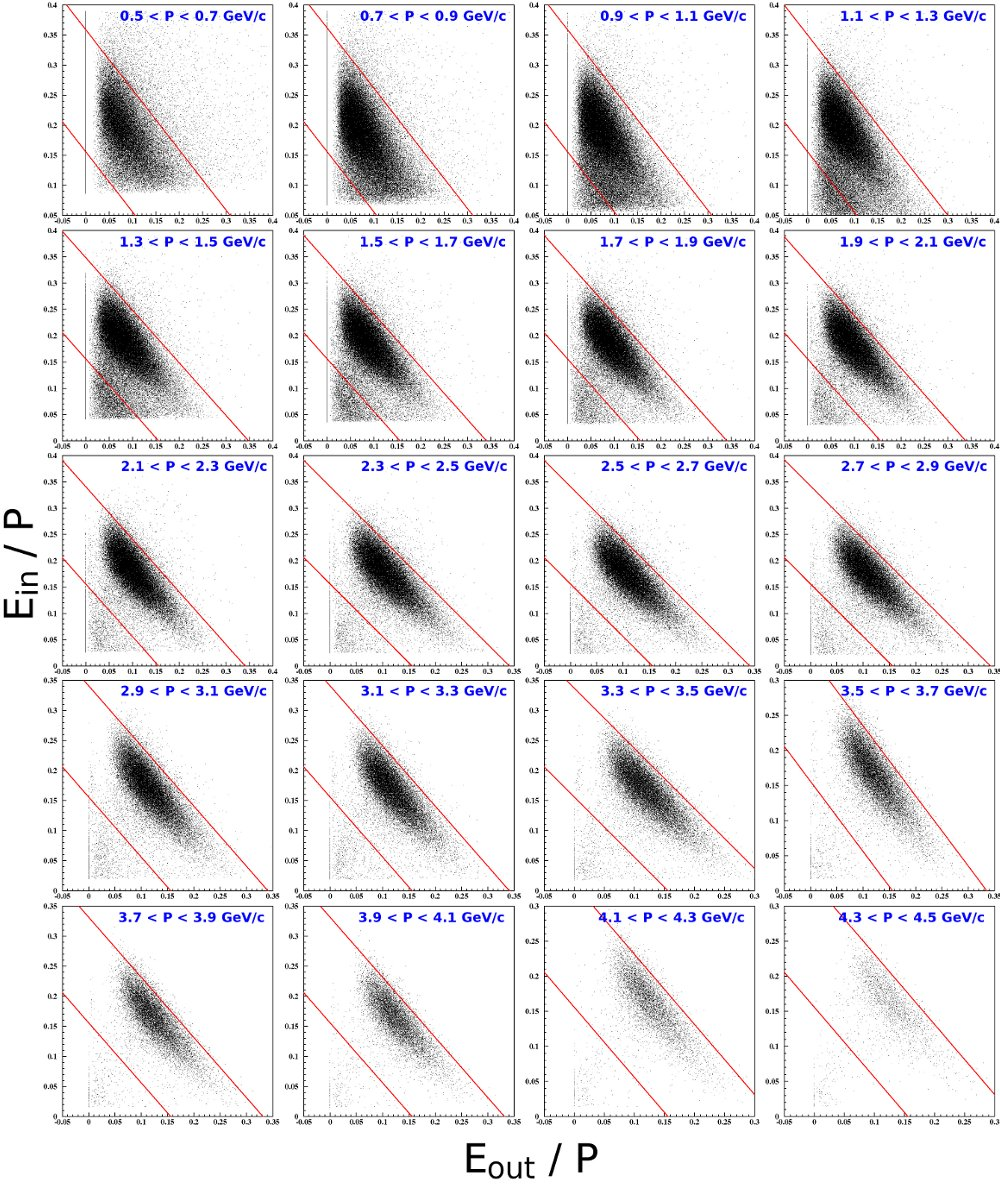
\includegraphics[width=14cm] {chap5-fig/fig02.jpg} 
\caption {Energy deposited in the inner part of the EC ($E_{in})$) as a function of the 
energy deposited in the outer part ($E_{out})$), both divided by the momentum of the 
particle. Each panel is for a different momentum range, the red lines 
illustrate the cuts from equation \ref{einout}.}
\label{eleEC}
\end{figure}

\begin{figure}[tbp]
\centering
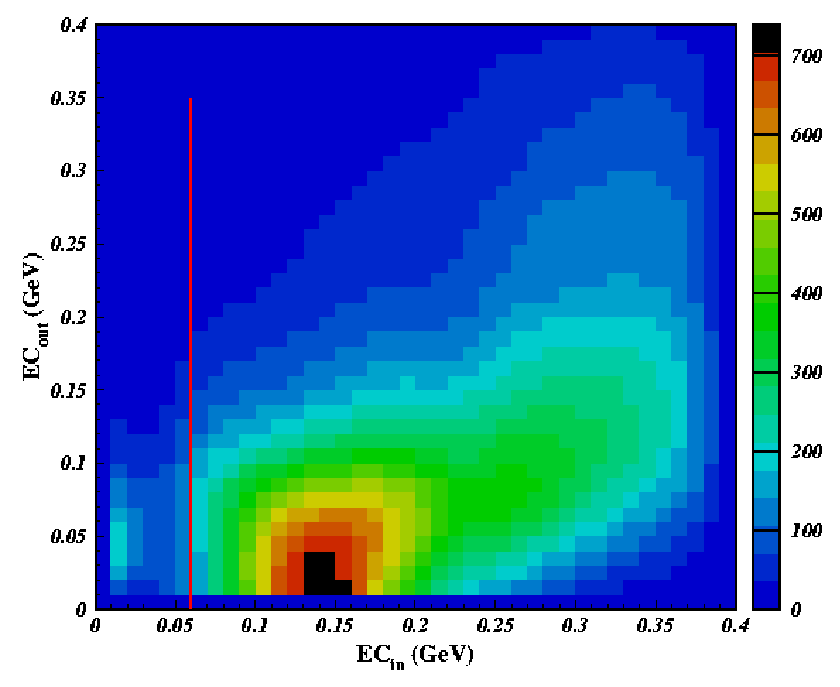
\includegraphics[width=9cm] {chap5-fig/fig03.png} 
\caption {Energy deposited in the inner part of the EC as a function of the 
energy in the outer part. The red line illustrates the cut applied for 
electron selection.}
\label{eleECi}
\end{figure}

In the CC, the mean number of photo-electrons\footnote{Photo-electrons are 
electrons produced in the front window of the Photo-Multiplier Tube (PMT) by 
single photons.} from a high energy electron is expected to be around 10.
However, hadrons can generate noise due to $\delta$ electrons produced in 
the materials of the detector. This signal is expected around 
one photo-electron, to remove it, we keep only tracks with more than 
2.5~photo-electrons (figure \ref{delta}). 

\begin{figure}[tbp]
\centering
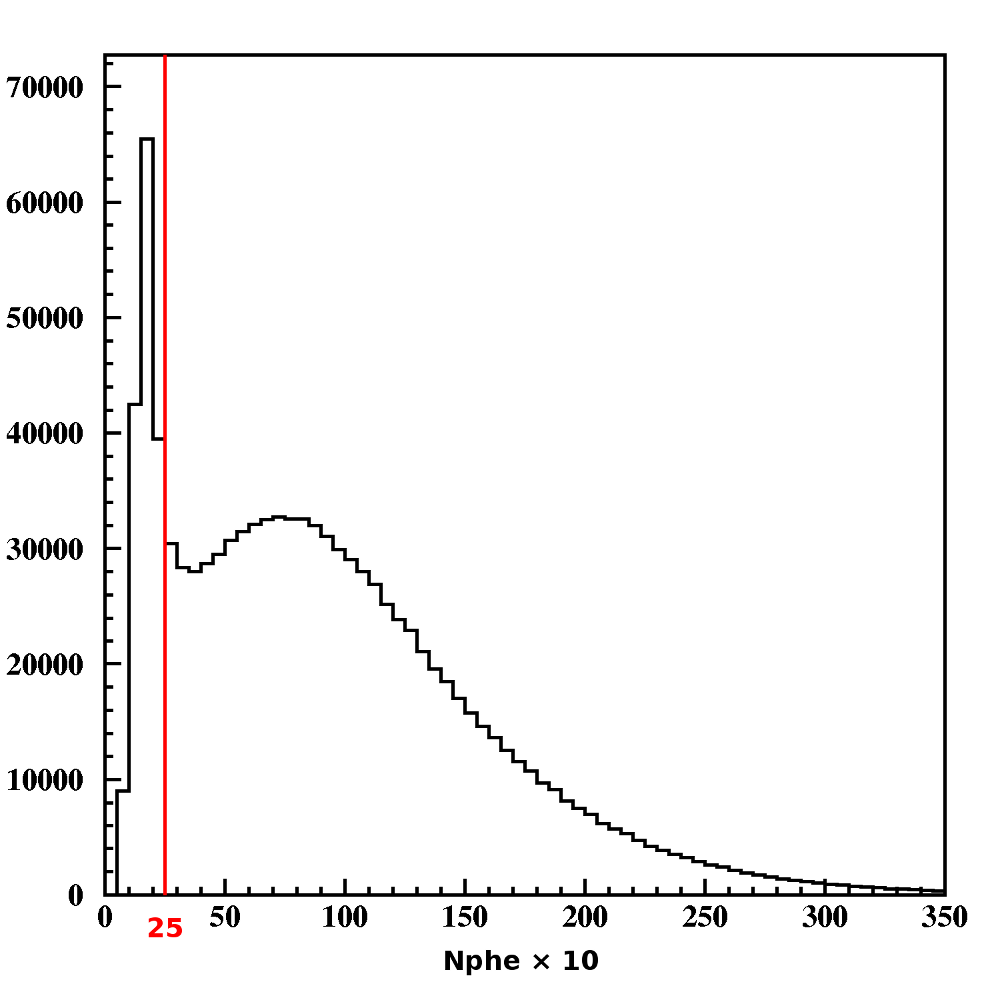
\includegraphics[width=8cm] {chap5-fig/fig04.png} 
\caption {Number of photo-electrons ($\times 10$) per tracks, the red line 
shows the cut to remove pion contamination.}
\label{delta}
\end{figure}

To select electrons, we also require that the particles are negatively charged, 
according to the bending direction of the tracks in the drift chamber.
Positively charged particles are identified as positrons. In the rest of the 
analysis we use events with only one electron and no positron to avoid any 
confusion between the scattered electron and electrons from hadronic decays or 
photon conversion to $e^+e^-$ pair, which often lead to the production of a
positron.

\subsubsection{$\pi^-$ Identification}
\label{PiId}

To identify negatively charged pions, we select negative tracks, which are not 
identified as electron. Pions are detected in the angular range from $\sim$10 to 
$\sim$140 degrees using the DC and SC only.

The identification consists mostly of a time of flight (TOF) test. We define 
$\Delta \beta = \beta_{measured} - {p \over \sqrt{p^2 + m_\pi^2}}$ and request 
$\Delta \beta$ to be zero within $\pm 0.03$. Figure \ref{PionTOF} illustrates 
the effect of this cut. We notice that there is not much negative kaons or 
anti-protons. Therefore, the contamination from these should be small (see 
section \ref{SysId} for more detailed analysis).

\begin{figure}[tbp]
\centering
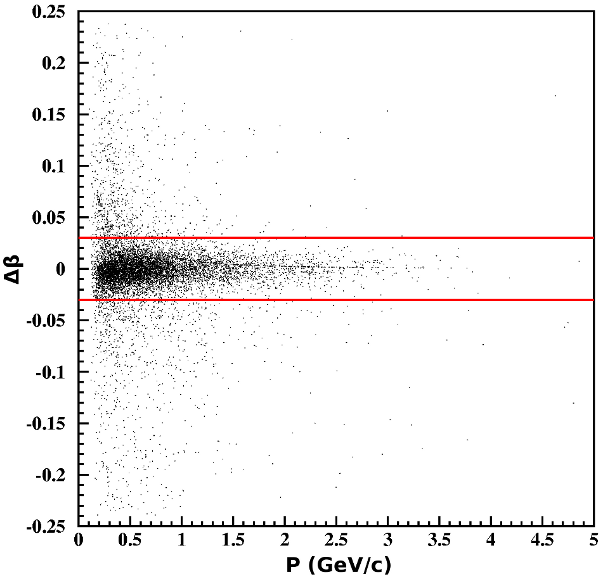
\includegraphics[width=8cm] {chap5-fig/fig05.png} 
\caption {$\Delta \beta$ as a 
function of momentum (GeV/c). Only negative particles are plotted. The red 
lines are the cuts applied to select negative pions.}
\label{PionTOF}
\end{figure}

In principle, pion identification could be improved using the Cherenkov counter 
for momentum higher than 2.5~GeV/c. But, the low efficiency observed (figure 
\ref{PionCC}), especially at momentum close to the threshold ($\sim$25\% at 
2.5~GeV/c and $\sim$50\% at 3~GeV/c), makes its use less compelling. 
Moreover, as only a very small amount of $K^-$ and no $\bar p$ are present on 
the figure \ref{PionTOF}, we decided not to use the CC for pion identification.

\begin{figure}[tbp]
\centering
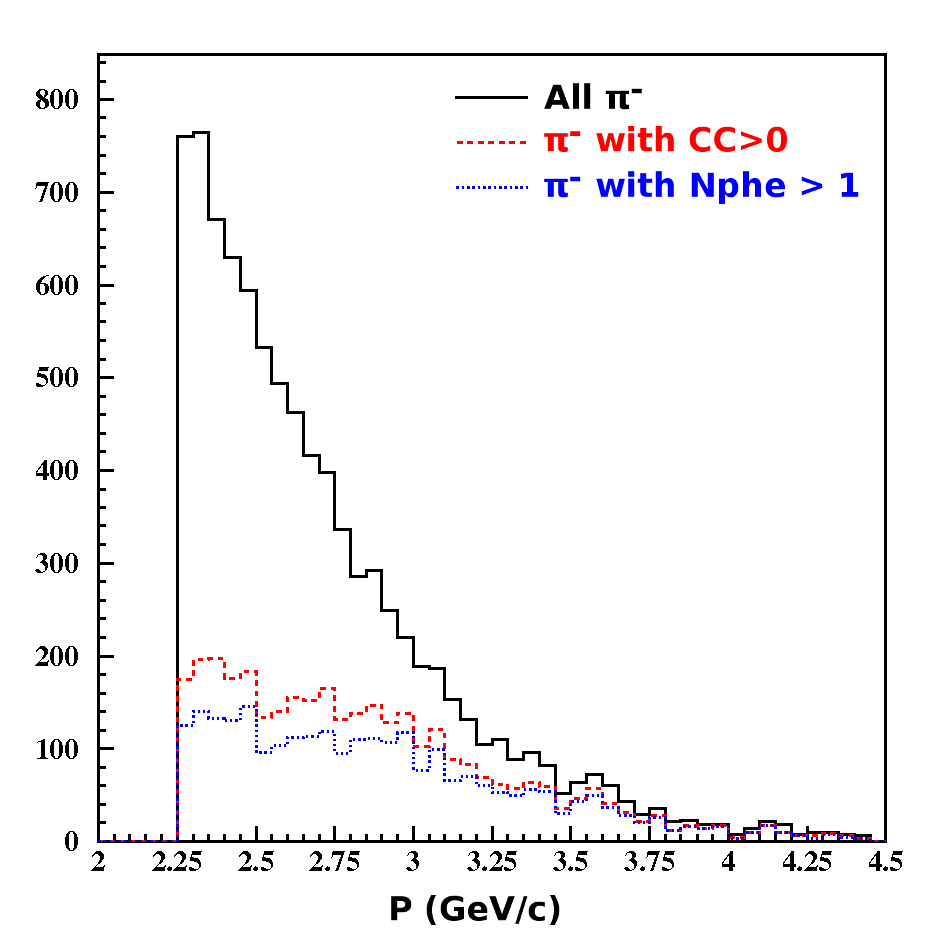
\includegraphics[width=8cm] {chap5-fig/fig06.png} 
\caption {Histograms of momentum (GeV/c) for $\pi^-$. In black are all 
identified $\pi^-$, in red pions that also fire in the Cherenkov counter and 
in blue those that fire in the Cherenkov counter with more than 
1 photo-electrons.}
\label{PionCC}
\end{figure}

\subsubsection{$\pi^+$ Identification}

The identification of positively charged pions is similar to that of negative 
pions. However, the time of flight plot is significantly more busy (figure 
\ref{PipTOF}), showing significant contamination from $K^+$ and protons at 
high momentum. As the CC is not efficient enough for hadron separation, the 
numerous kaons and protons should be removed by a tighter TOF cut:

\begin{subequations}\label{TOF-Pip}
\begin{align}
    p_\pi &\leq 3.375 \text{ GeV/c : }
  & \Delta \beta &> \max\left(-0.03,{p \over\sqrt{p^2+0.4^2}}\right), \\ 
    p_\pi &> 3.375    \text{ GeV/c : }
  & \Delta \beta &> \max\left(-0.02,{p \over\sqrt{p^2+0.7^2}}\right).
\end{align}
\end{subequations}

These cuts permit to minimize the kaon contamination, below 2.5~GeV/c, and the 
proton contamination for all momentum. The kaon contribution cannot be avoided, however 
it should remain a small contribution ($\sim$ 3\% according to simulation) 
with only a small effect on the final results (see section \ref{SysId} 
for details). Because protons could lead to even more contamination than kaons, 
a stricter cut is used at high momentum. This cut is also justified by 
HERMES data \cite{Airapetian:2007vu}, which show a very 
different behavior of the protons compared to the other hadrons (see chapter \ref{chap:data}).

\begin{figure}[tbp]
\centering
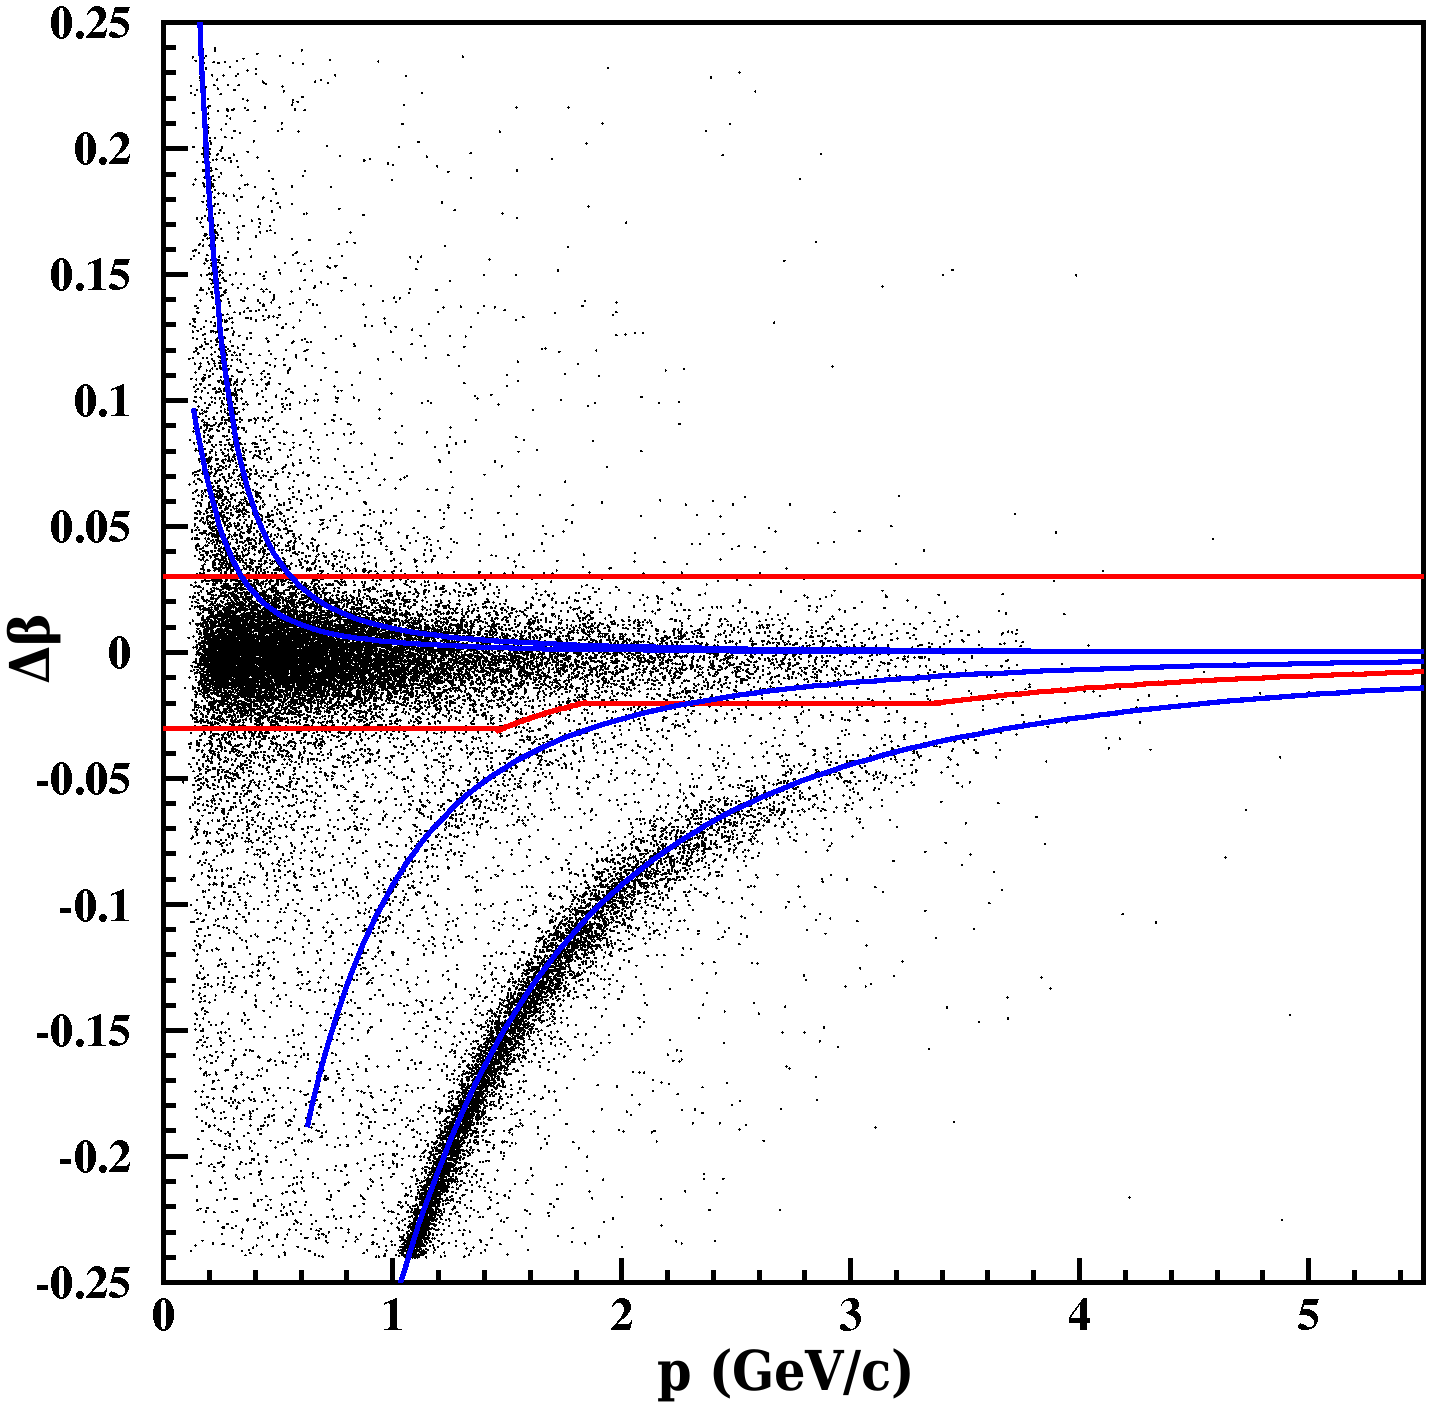
\includegraphics[width=8cm] {chap5-fig/pip_data.png} 
\caption {$\Delta \beta$ as a 
function of momentum (GeV/c). Only positive particles are shown, the red 
lines are the cuts applied to select positive pions. The blue lines indicate 
theoretical positions for other particle masses, are plotted from top to 
bottom the lines for positrons, muons, kaons and protons.}
\label{PipTOF}
\end{figure}

\subsubsection{Target Determination}

To differentiate the two targets and remove the background, we need to 
determine the origin of the particles. It appears that the different sectors 
are shifted in $z$ (figure \ref{vertex}), because of a small misalignment of 
the beam with the detector. To correct this problem, we apply the modification shown in table 
\ref{tab:vertex} for the vertex determination. Those values were determined by 
fitting the solid target position viewed by each sector.

\begin{table}[p]
  \centering
  \begin{tabular}{@{} cc @{}}
    \hline
    Sector & Shift (cm) \\ 
    \hline
    1 & + 0.1 \\ 
    2 & - 0.4 \\ 
    3 & - 0.6 \\ 
    4 & - 0.1 \\ 
    5 & + 0.4 \\ 
    6 & + 0.6 \\ 
    \hline
  \end{tabular}
  \caption{Values used to correct the vertex information for all sectors}
  \label{tab:vertex}
\end{table}

The position of the targets may also vary from one run to another, but 
this does not happen too often. Indeed, except for aluminum, the targets remain in 
the same position within one or two millimeters. The positions, in CLAS 
coordinates, are given in table \ref{tab:targets}.

\begin{table}[p]
  \centering
  \begin{tabular}{|c|c|c|c|c|c|c|}
    \hline
    Target & Carbon & Al (1) & Al (2) & Iron   & Tin    & Lead   \\ 
    \hline \hline
    Liquid & -30.1  & n/a    & n/a    & -30.2  & -30.1  & -30.1  \\ 
    Solid  & -24.7  & -25.0  & -23.8  & -24.9  & -23.8  & -24.9  \\
    \hline
  \end{tabular}
  \caption{Measured mean vertex position of targets, relative to the center of 
           CLAS (in cm). (Aluminum data are separated in two sets because the 
           target position appears to have changed at some point.)}
  \label{tab:targets}
\end{table}

\begin{figure}[p]
\centering
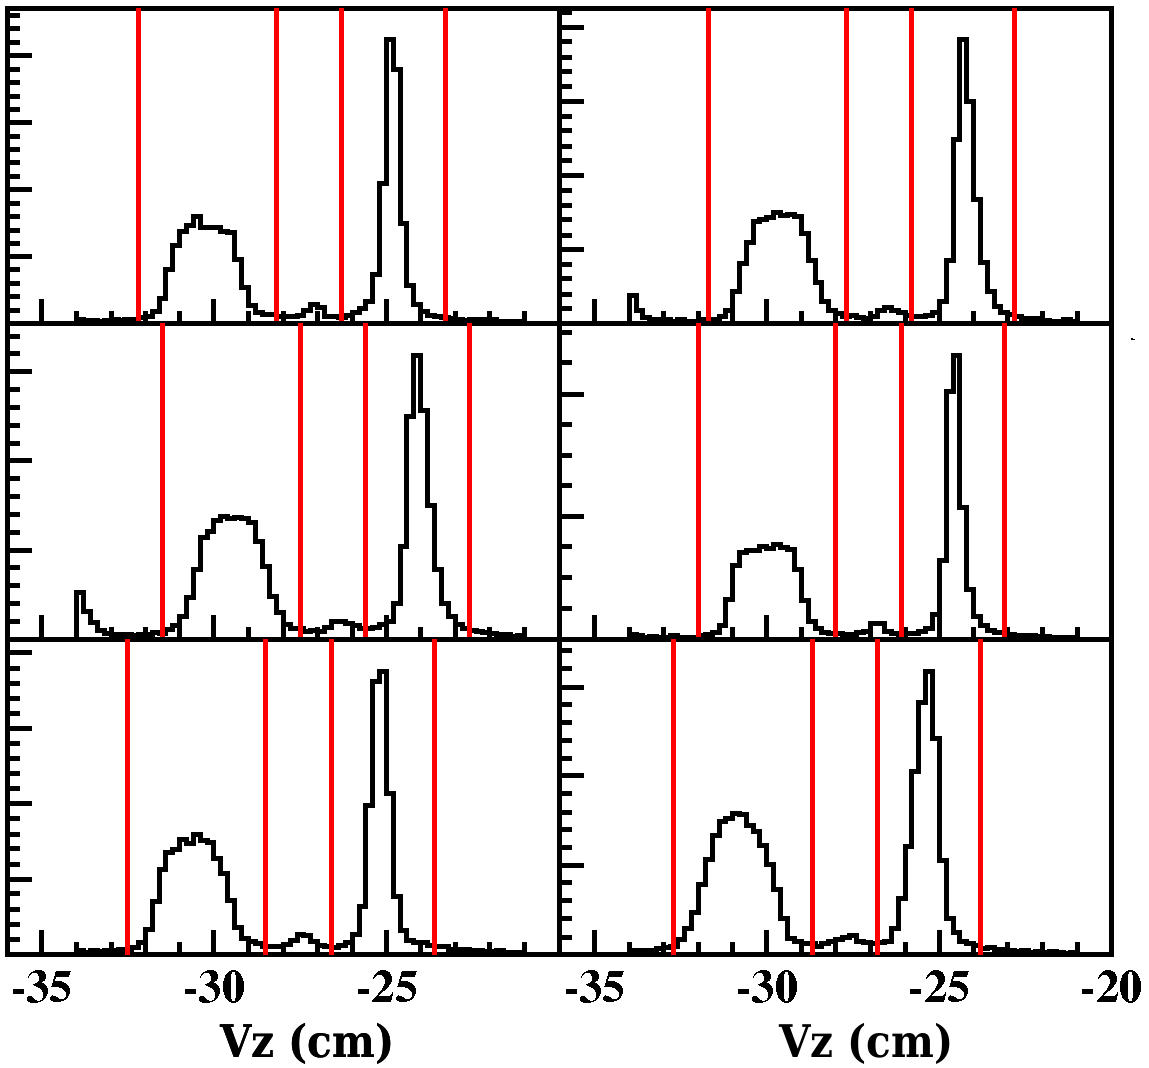
\includegraphics[width=10cm] {chap5-fig/Vertex_el_data.png}
\caption {In each sector, the reconstructed vertex of electrons along the beam
direction relatively to the center of CLAS. The red lines show the cuts 
to select the targets.}
\label{vertex}
\end{figure}

The detected electrons are associated with the solid target if their vertex 
position is at less than 1.5~cm ($\sim$3~$\sigma$) from the value of table 
\ref{tab:targets}. For the liquid target, the cut is larger, 2 cm, in order to 
account for the size of the target (see figure \ref{vertex}). The vertex of 
the pions is checked against the electron one and we request that 
$| Vz^{e^-} - Vz^{\pi} | < 3$ cm (see figure \ref{fig:dvzpi}).

\begin{figure}[tbp]
\centering
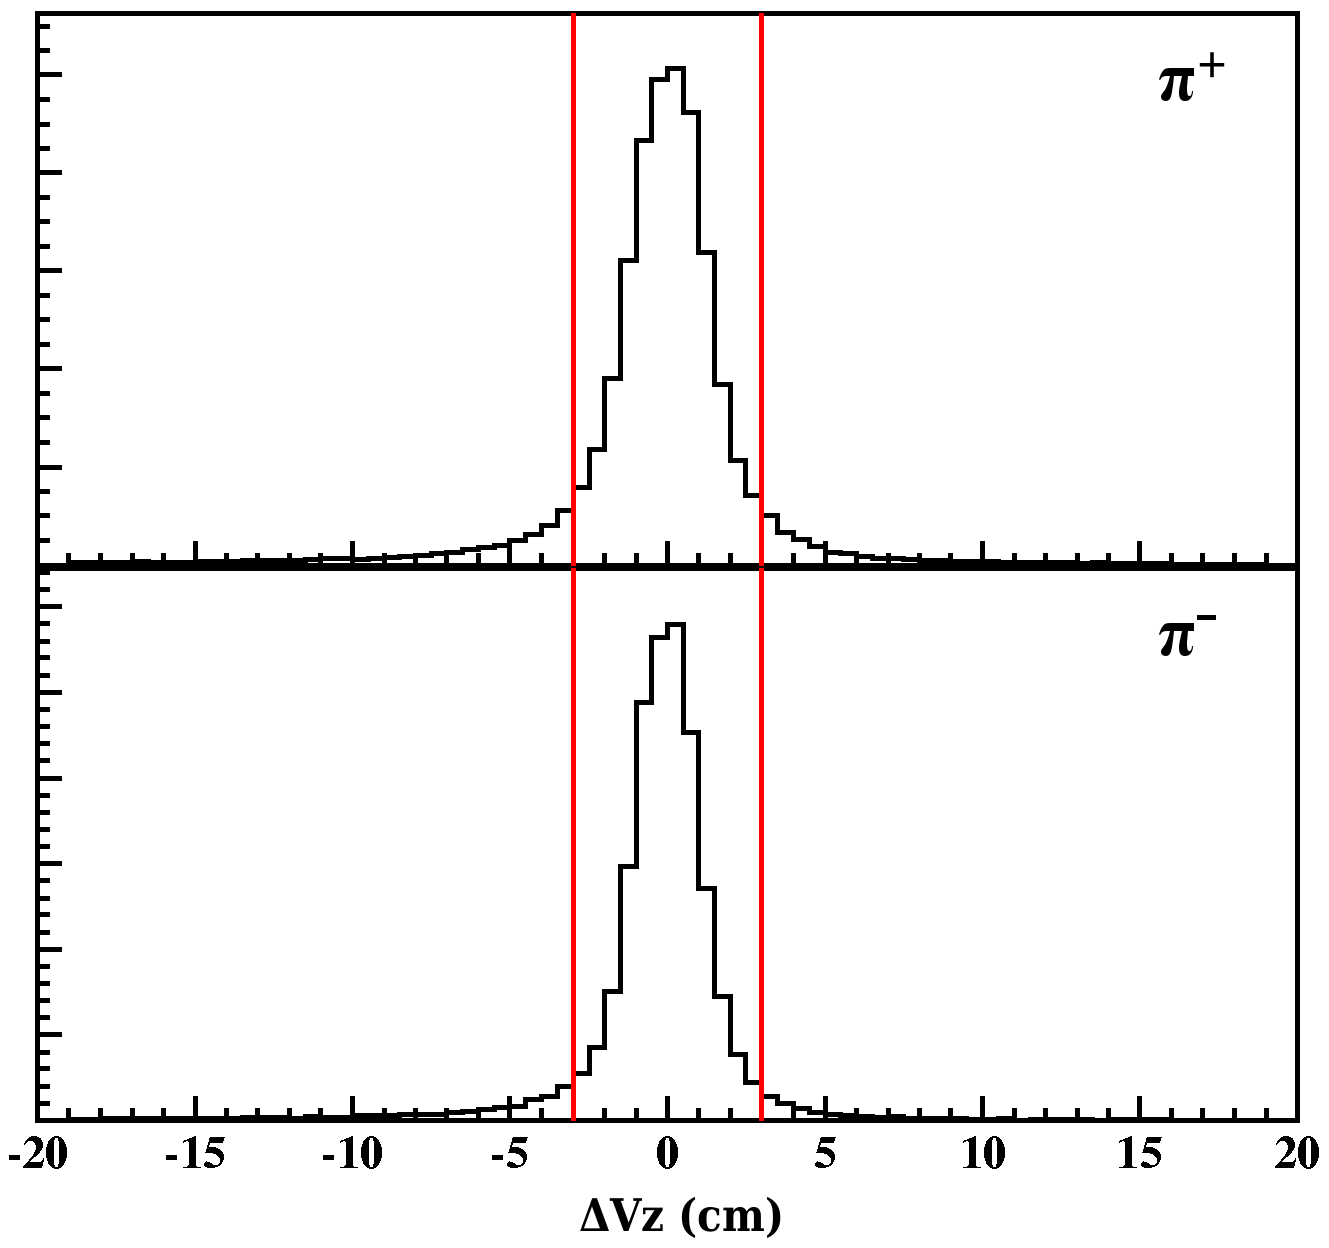
\includegraphics[width=8cm] {chap5-fig/Vertex_pi_data.png}
\caption {Distance along the beam axis between the electrons and pions 
vertexes. $\pi^+$ are plotted in the top panel and the $\pi^-$ in the bottom.
The red lines show the cuts applied to select pions.}
\label{fig:dvzpi}
\end{figure}

\subsubsection{Data Quality}

To check the quality of the runs\footnote{Runs correspond roughly to two hours
of data, they can be smaller in case of problem.}, we look at the ratio of the number of 
scattered electrons, between the liquid and solid targets. If the beam is 
hitting other materials than the targets or if the detector is not working 
properly this ratio can be off and indicates a problematic run. The figure 
\ref{DataQ} shows the values obtained; we fit the 
mean value for all runs of each target and eliminate runs away by more than 
5$\sigma$. We note that the ratios are coherent with target thicknesses given 
in \cite{Hakobyan:2008zz} except for carbon. Because of this, the density of 
the carbon target was remeasured recently and found to be coherent with the 
data\footnote{i.e. (1.747+/-0.0007)g/cm$^3$ instead of 2.235 g/cm$^3$}.

\begin{figure}[tbp]
\centering
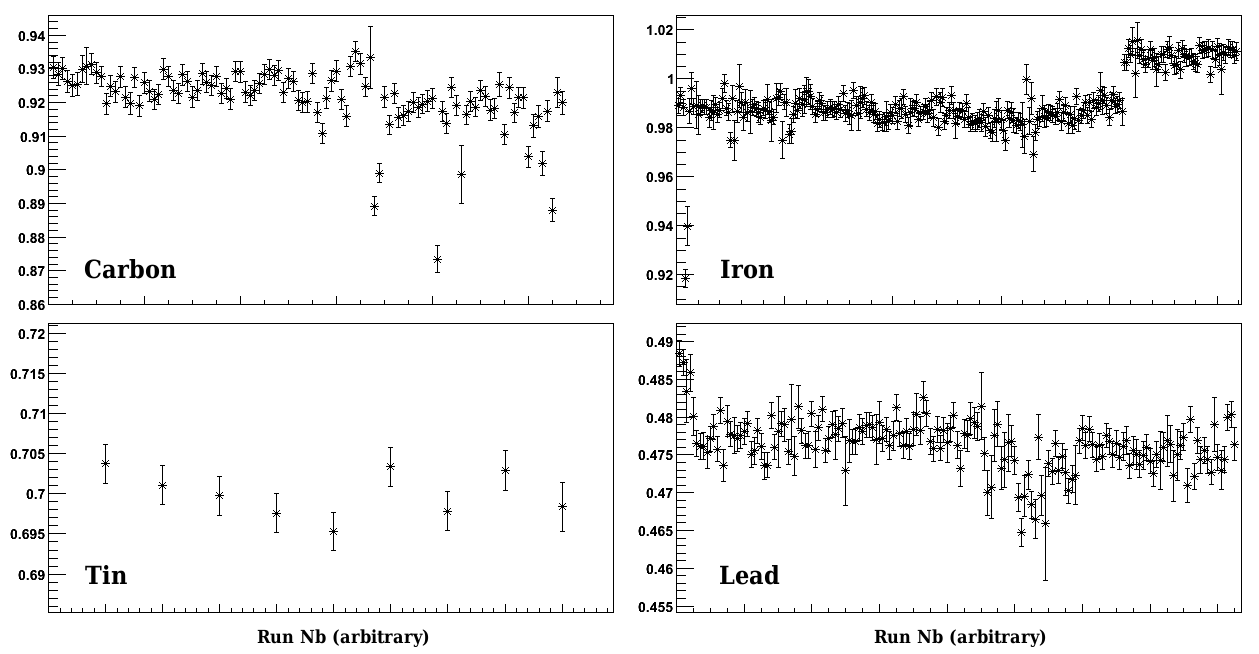
\includegraphics[width=15cm] {chap5-fig/TargetElRatio.png}
\caption {Ratio of the number of electrons scattered by the targets (solid over deuterium) 
for each run.}
\label{DataQ}
\end{figure}

\subsection{Extraction of Multiplicity Ratio and $\Delta$P$_\perp^2$}
\label{sec:obs}

Since we are interested in deep inelastic scattering, we use the following 
cuts: $Q^2 > 1$~GeV$^2$/c$^2$ and $W > 2$~GeV. We also apply a cut $y < 0.85$ to 
reduce the impact of radiative effects, which will be discussed in more details in 
the section \ref{RadCor}.

\subsubsection{Method}
\label{RatioCalc}

Once the identification is done, the calculation of the observables is 
straight forward and the statistical errors are calculated with this expression

\begin{equation}
{\delta \left ( R_A^h \right ) \over R_A^h} = \sqrt{ 1 /N_A^h + 1/ N_A^e +1/N_D^h + 1/N_D^e}
\end{equation}
and
\begin{equation}
\left ( \delta \left ( \Delta \langle P_\perp^2 \rangle \right ) \right )^2 = 
   \left ({\langle P_\perp^4 \rangle - \langle P_\perp^2 \rangle ^2}\right )_A / N_A^h
 + \left ({\langle P_\perp^4 \rangle - \langle P_\perp^2 \rangle ^2}\right )_D / N_D^h.
\end{equation}

The implementation of acceptance and radiative corrections is done through weights
given to each particles depending on its kinematic. The multiplicity ratio becomes

\begin{equation}
R_A^h (Q^2,\nu,z_h,P_\perp^2) = {{\sum \omega_A^h (Q^2,\nu,z_h,P_\perp^2) / \sum \omega_A^e (Q^2,\nu)} 
                       \over {\sum \omega_D^h (Q^2,\nu,z_h,P_\perp^2) / \sum \omega_D^e (Q^2,\nu)}},
\end{equation}
with $\omega$ the weights and all the sums running over all measured particles.
The expression for the transverse momentum broadening remains
\begin{equation}
\Delta \langle P_\perp^2 \rangle = \langle P_\perp^2 \rangle_A - \langle P_\perp^2 \rangle_D,
\end{equation}
but with
\begin{equation}
\langle P_\perp^2 \rangle = {\sum P_\perp^2 \times \omega (Q^2,\nu,z_h,P_\perp^2) \over \sum \omega (Q^2,\nu,z_h,P_\perp^2)}.
\end{equation}

This expressions leads to new expressions for the statistical error uncertainties: 

\begin{equation}
{\delta \left ( R_A^h \right ) \over R_A^h} = 
      \sqrt{ \left ( {\sum {\omega^h_A}^2 \over \left (\sum \omega^h_A \right )^2} \right ) 
           + \left ( {\sum {\omega^e_A}^2 \over \left (\sum \omega^e_A \right )^2} \right ) 
           + \left ( {\sum {\omega^h_D}^2 \over \left (\sum \omega^h_D \right )^2} \right ) 
           + \left ( {\sum {\omega^e_D}^2 \over \left (\sum \omega^e_D \right )^2} \right ) }
\end{equation}
 and 
\begin{equation}
\begin{split}
\left ( \delta \left ( \Delta \langle P_\perp^2 \rangle \right ) \right )^2 = 
   \left ({{\sum \omega^h_A P_\perp^4 }\over{\sum \omega^h_A}} - \left ({\sum \omega^h_A P_\perp^2 }\over{\sum \omega^h_A}\right )^2 \right ) 
         \times \left ( {\sum \left ( {\omega^h_A}^2 \right ) \over \left ( \sum \omega^h_A \right ) ^2 }\right ) \\
 + \left ({{\sum \omega^h_D P_\perp^4 }\over{\sum \omega^h_D}} - \left ({\sum \omega^h_D P_\perp^2 }\over{\sum \omega^h_D}\right )^2 \right ) 
	 \times \left ( {\sum \left ( {\omega^h_D}^2 \right ) \over \left ( \sum \omega^h_D \right ) ^2 }\right ).
\end{split}
\end{equation}

\subsubsection{Preliminary Results}
\label{prelim}

We present in figure \ref{fig:prelim} few preliminary results, before the application of any correction, with the goal to 
provide a first idea on data quality. The preliminary results will also be used to 
illustrate the effects of the corrections discussed below.

\begin{figure}[htb]
\centering
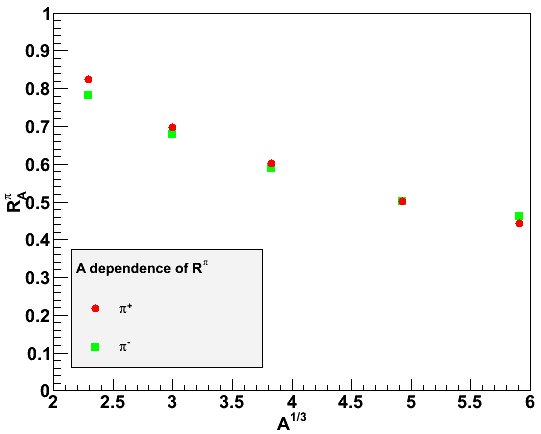
\includegraphics[width=7.4cm] {chap5-fig/a_RvA.png} 
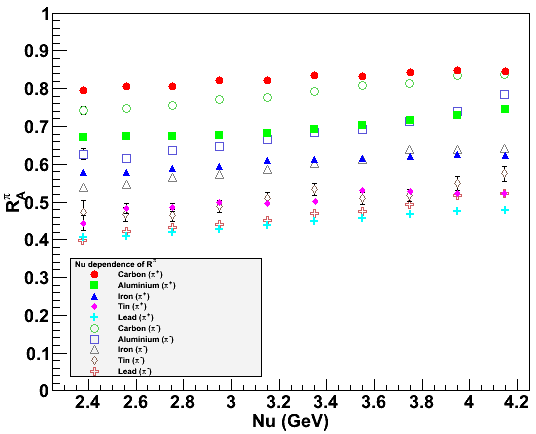
\includegraphics[width=7.4cm] {chap5-fig/a_RvZ.png} 
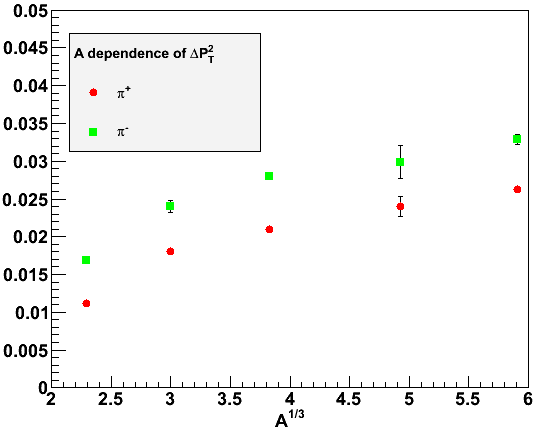
\includegraphics[width=7.4cm] {chap5-fig/a_PvA.png} 
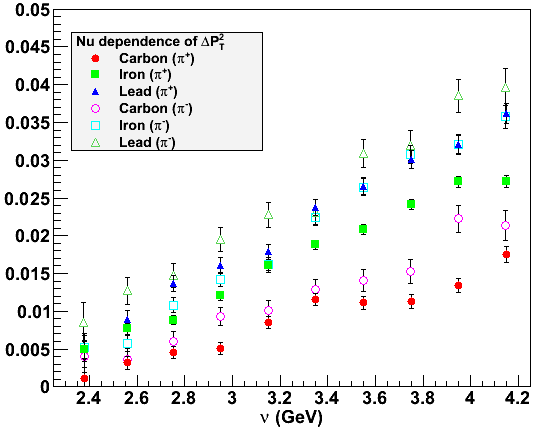
\includegraphics[width=7.4cm] {chap5-fig/a_PvNu.png} 
\caption {Results for multiplicity ratios (top) and transverse momentum 
broadening (bottom) without correction.}
\label{fig:prelim}
\end{figure}


\subsection{Corrections}
\label{sec:corrections}

\subsubsection{Acceptance Correction}
\label{sec:accept}

The acceptance correction consists of applying weights to the events in 
experimental data to correct for the inefficient parts of the detectors.
Incidentally, it also corrects for small other issues of detection,
such as misidentification and scattering on detectors materials. The quality 
of the correction depends on the ability of the simulation to reproduce the 
experiment, the statistics accumulated and the size of interfering effects, such 
as bin migration.

\paragraph{Simulation}
\label{sec:simul}

To correct for acceptance effects, we simulated a total of a 100 million events 
per target ($^2$H, C, Fe and Pb) using the PYTHIA \cite{Sjostrand:2006za} 
event generator slightly modified to include Fermi motion effects. The 
generated events are processed by the CLAS software (GSIM, GPP and user\_ana) 
to simulate the detector and the reconstruction process similarly to the one for experimental data.

Then the simulated data are processed in a similar way than the experimental data by 
applying the cuts described in the section \ref{sec:pid}. Overall the 
simulation reproduces quite well the detectors responses, yet two issues might 
affect us and have to be understood. First, the efficiency of the CC is overestimated in the simulation. 
On the electron side the signal is a little stronger in the simulation (11 
photo-electrons) compared to experimental data (8 photo-electrons), but this 
feature should not affect us too much, because we are cutting only the tail of the 
distribution in both cases. For pion identification, as mentioned in section \ref{PiId},
we do not use the CC because of its unexpectedly low efficiency 
We observe, in the simulation, a much better detector response than in experiment 
(figure \ref{simPionCC} compared to figure \ref{PionCC}), this result also advocates against the use of the CC in the 
particle identification. Indeed, the poor reproduction of the experimental signal would introduce a bias in our acceptance correction. 
Second, in figure \ref{vertex} the cuts on vertex are shifted from one sector 
to another, since the simulation have perfect alignment of beam with CLAS this 
feature is not present in the simulated data. Therefore, we do not apply the 
shift from the table \ref{tab:vertex} to the simulation; results are shown in 
figure~\ref{simvertex}.

\begin{figure}[tpb]
\centering
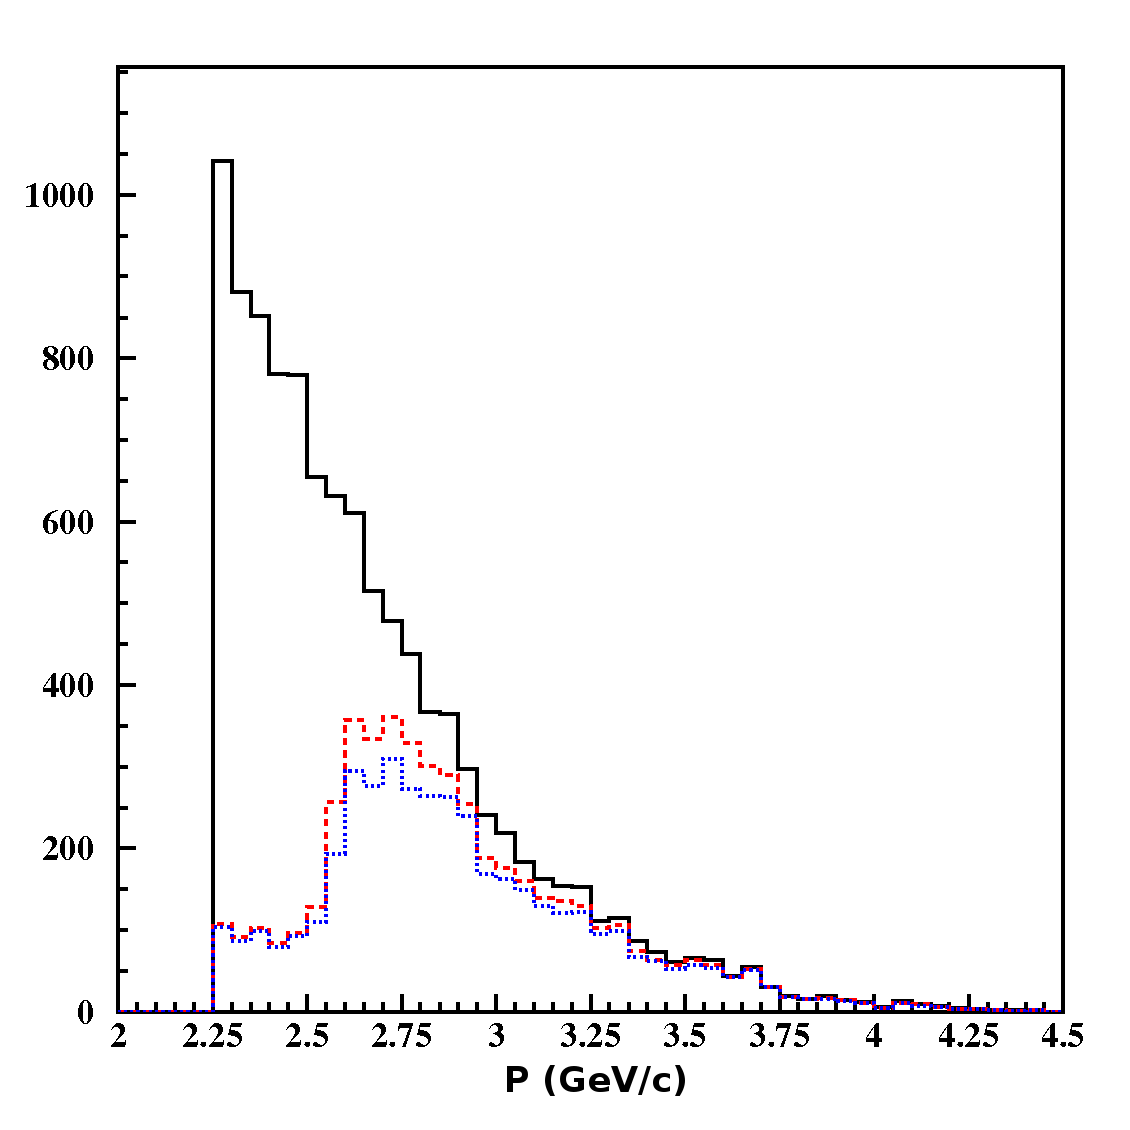
\includegraphics[width=9cm] {chap5-fig/fig06simul.png} 
\caption {Histograms of momentum (GeV/c) of $\pi^-$ for {\bf simulated data}.
In black are all identified $\pi^-$, in red pions that also fire in the 
Cherenkov counter and in blue those that fire in the Cherenkov counter with 
more than one photo-electron.}
\label{simPionCC}
\end{figure}

\begin{figure}[tpb]
\centering
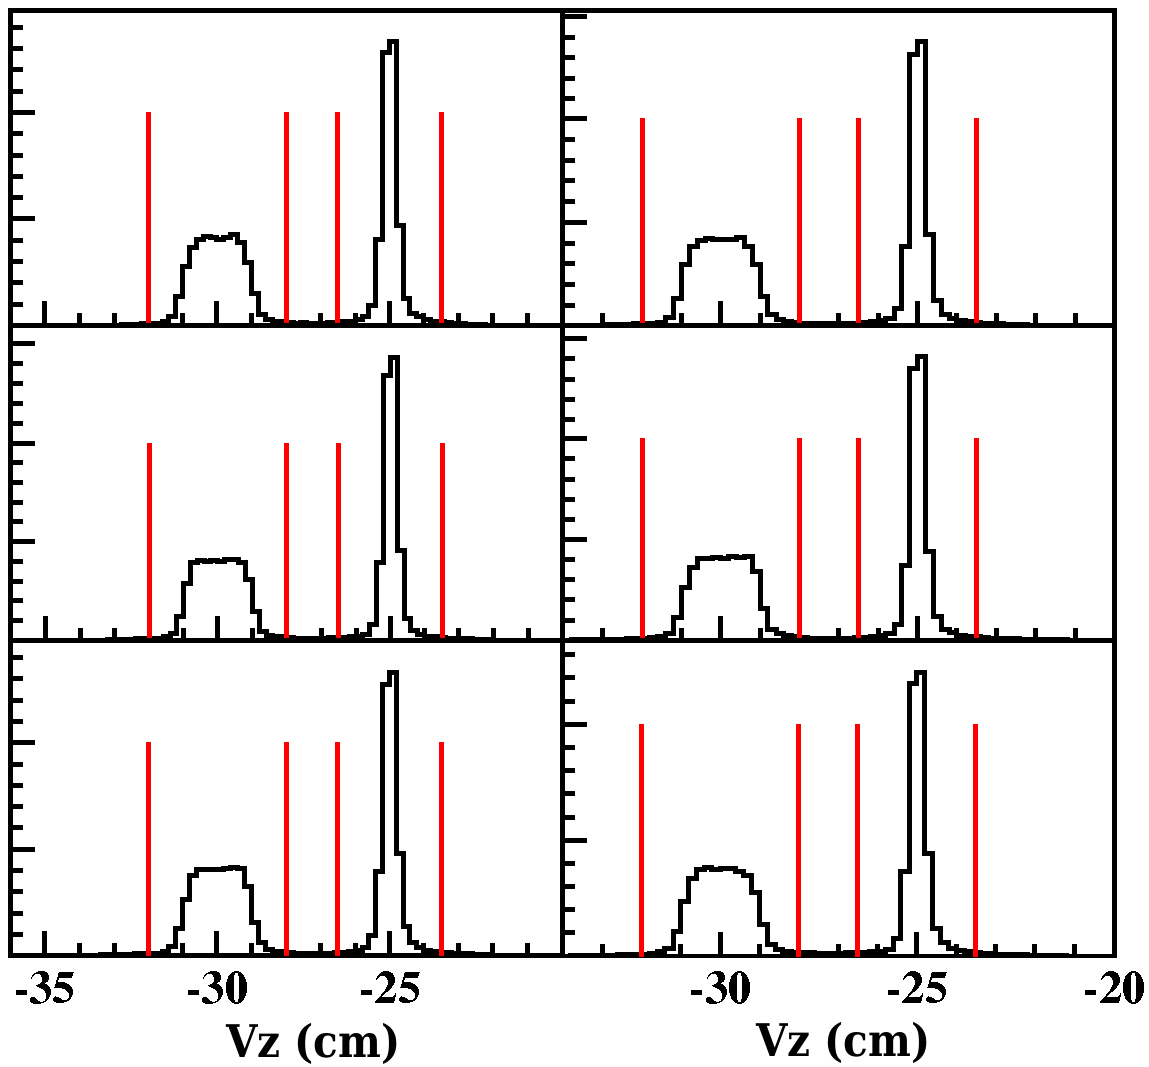
\includegraphics[width=9cm] {chap5-fig/Vertex_el_sim.png}
\caption {Reconstructed vertex position, along the beam direction, with values 
relative to CLAS center, for electrons from {\bf simulated data} and each 
sector. The red lines show the cuts used to select the targets.}
\label{simvertex}
\end{figure}

The kinematic distributions from the simulation are compared to the 
experimental ones. This is important for the acceptance correction, to see 
whether or not, we can integrate over these variables for the correction.
Comparisons between simulation and experiment are shown in figures 
\ref{fig:compNuQ2} to \ref{fig:compPhih}. The agreement is reasonable, but not 
perfect. The differences are due to the PYTHIA simulation, which is not including some 
physical effects, such as radiative and diffractive processes.

\begin{figure}[tbp]
\centering
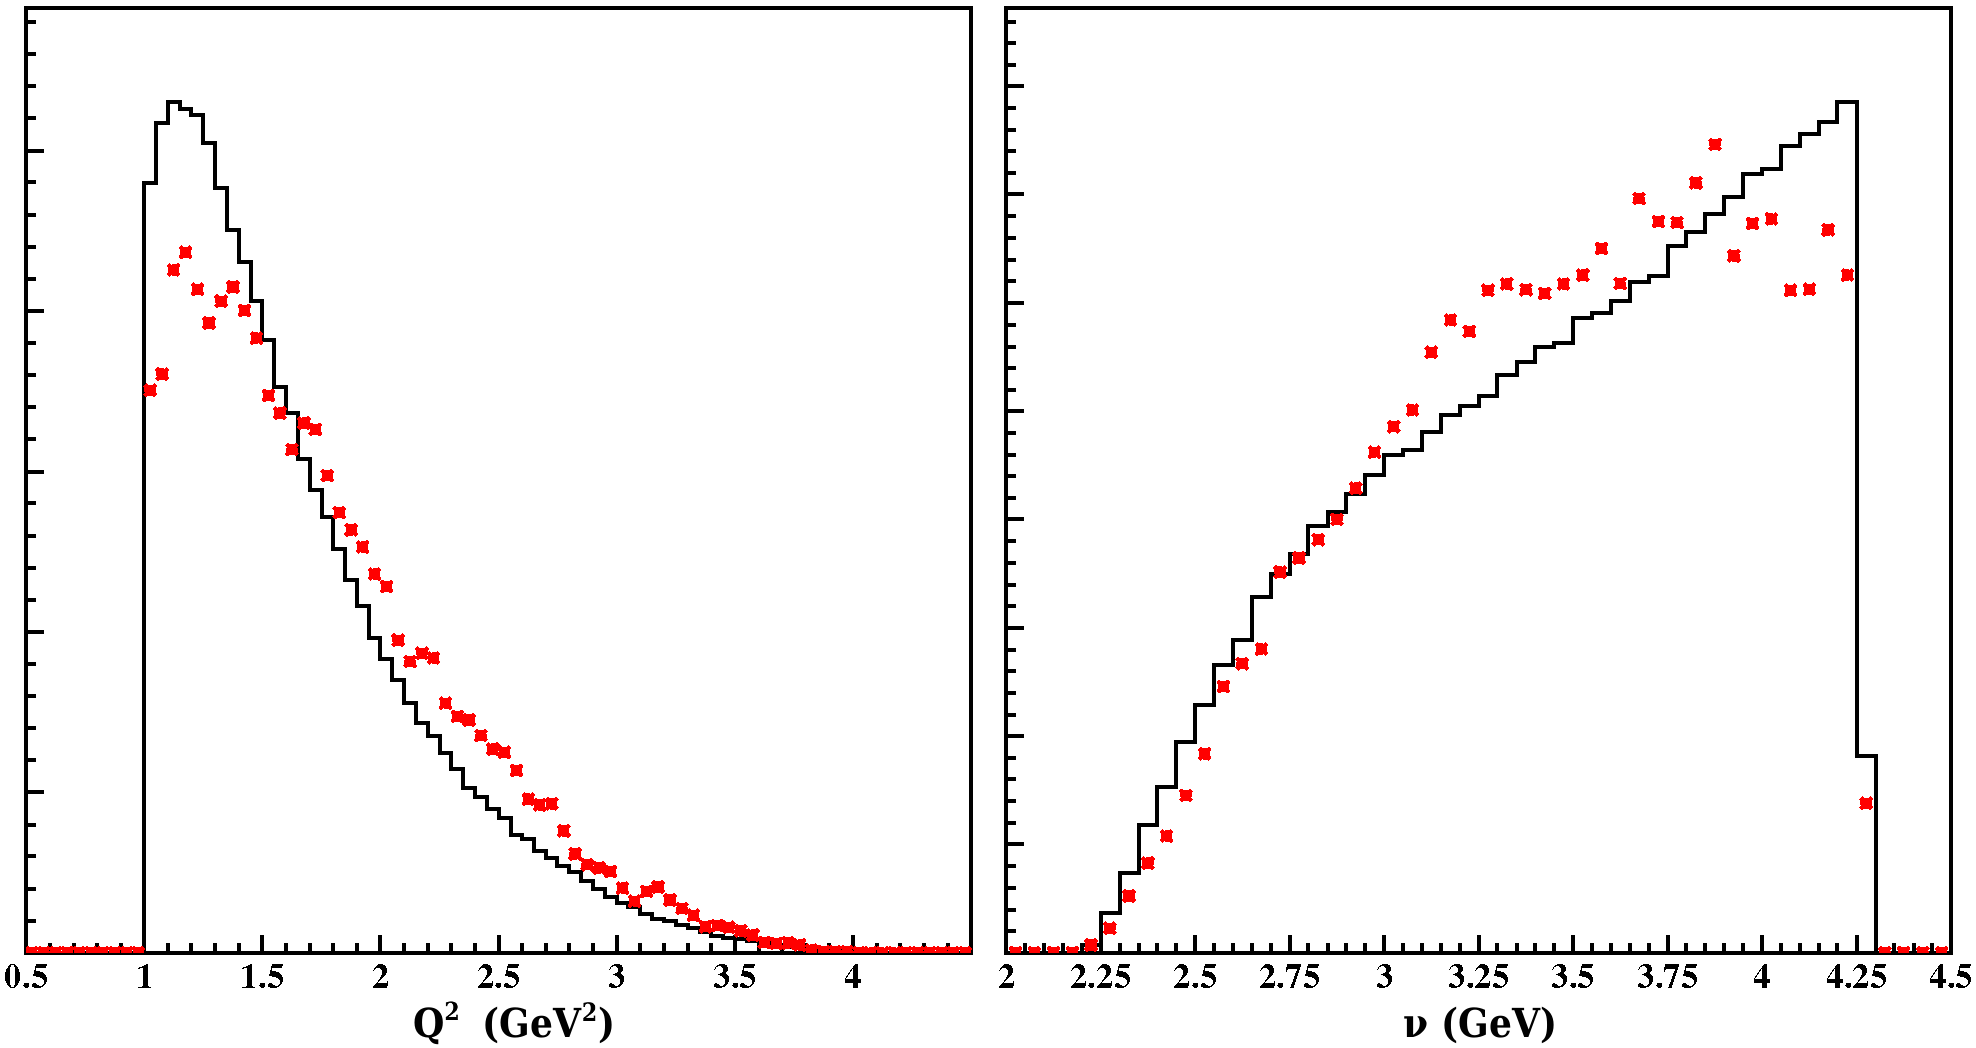
\includegraphics[width=12cm] {chap5-fig/El_compar.png}
\caption {Comparisons, for $Q^2$ (GeV$^2$/c$^2$) and $\nu$ (GeV), of the distributions
from simulated (red crosses) and experimental (histogram) data using deuterium target.}
\label{fig:compNuQ2}
\end{figure}

\begin{figure}[tbp]
\centering
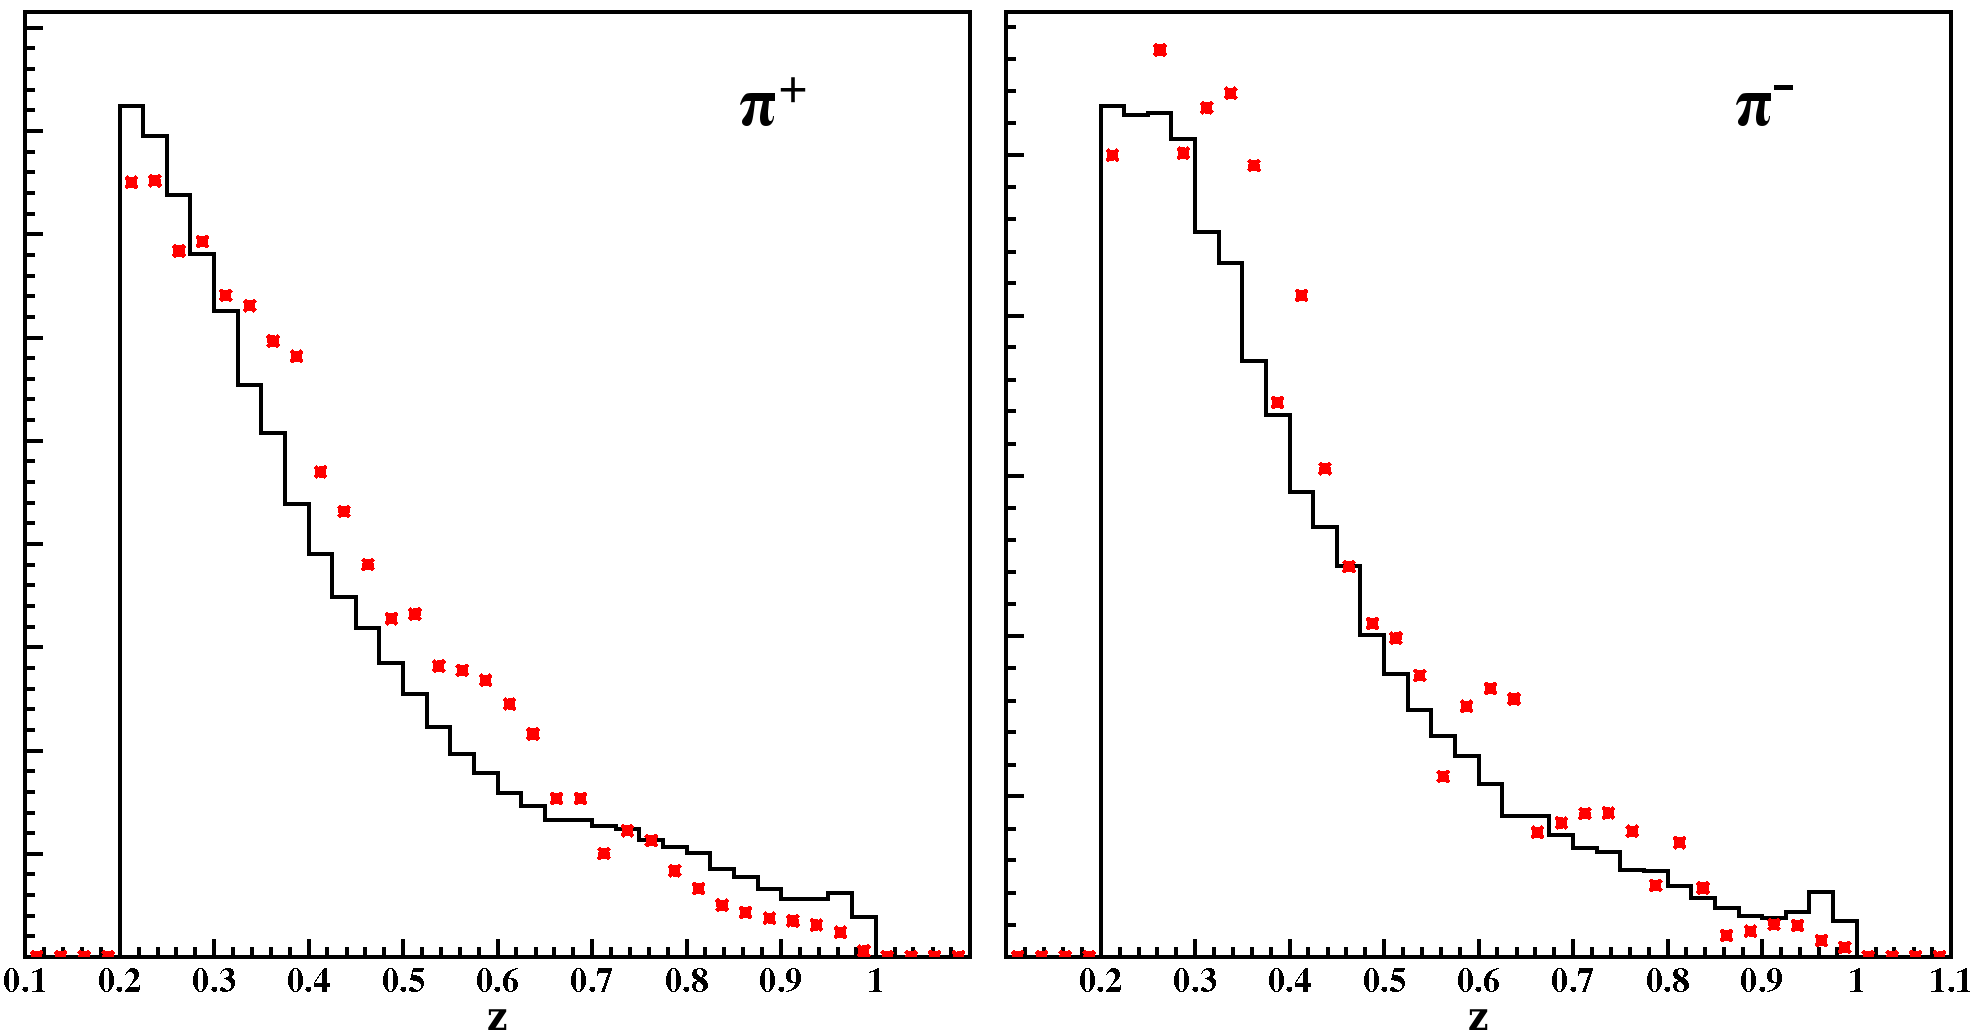
\includegraphics[width=12cm] {chap5-fig/z_compar.png}
\caption {Comparisons, for $z$ of charged pions, of the distributions
from simulated (red crosses) and experimental (histogram) data using deuterium target.}
\label{fig:compZ}
\end{figure}

\begin{figure}[tbp]
\centering
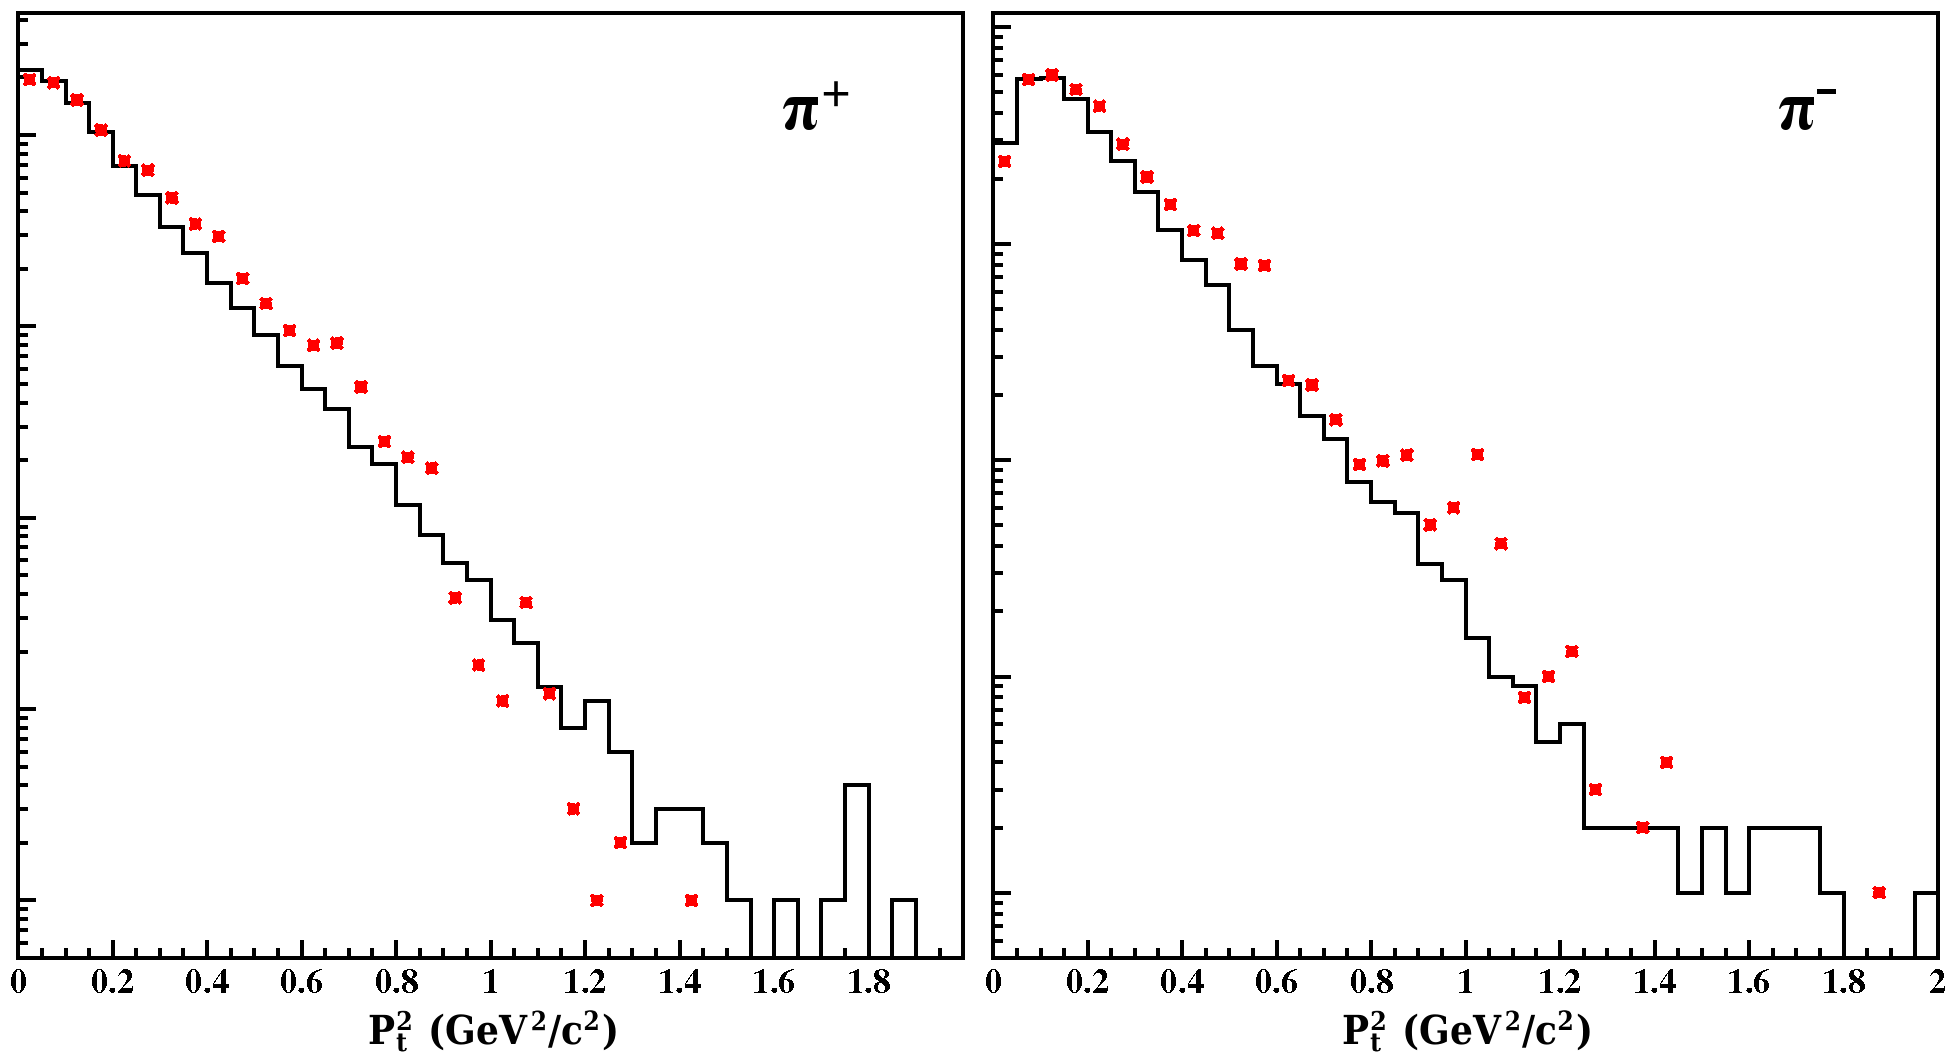
\includegraphics[width=12cm] {chap5-fig/pts_compar.png}
\caption {Comparisons, for \pt (GeV$^2$/c$^2$) of charged pions, of the distributions
from simulated (red crosses) and experimental (histogram) data using deuterium target.}
\label{fig:compPts}
\end{figure}

\begin{figure}[tbp]
\centering
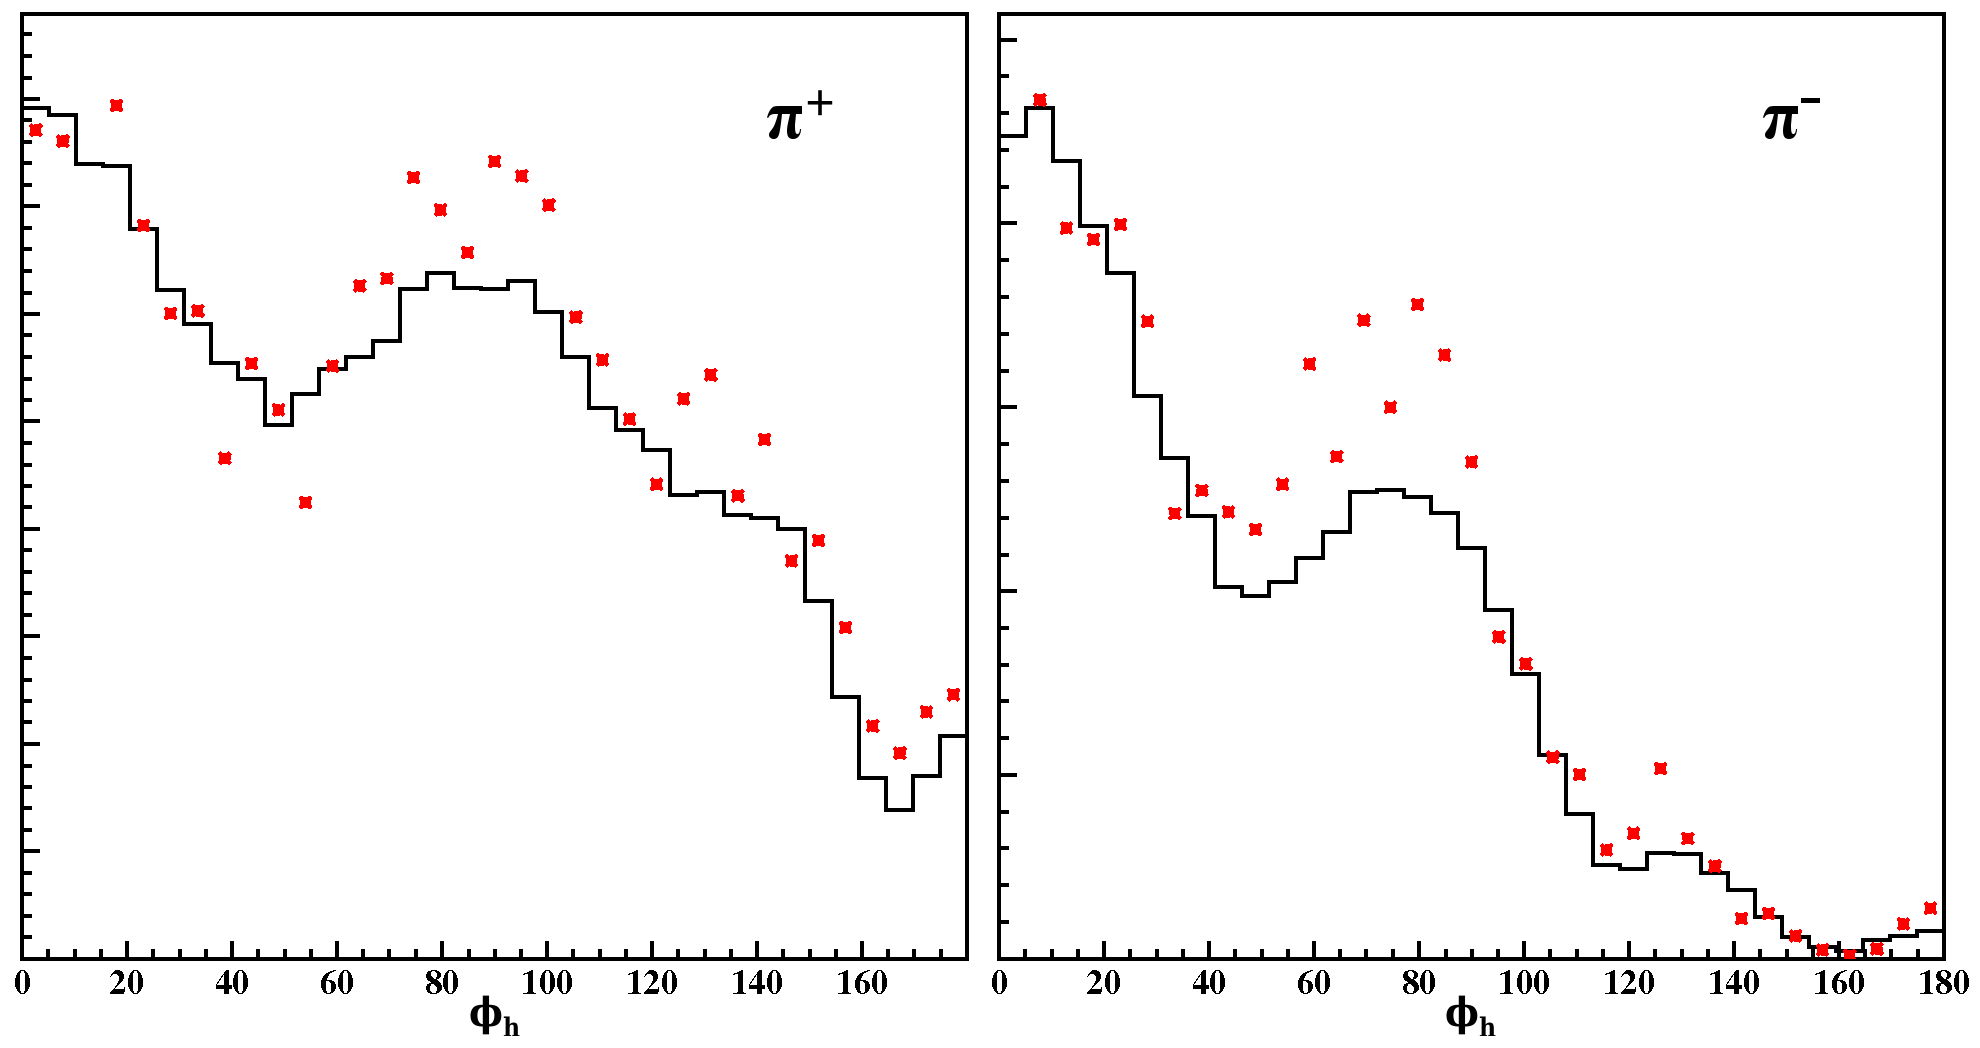
\includegraphics[width=12cm] {chap5-fig/phih_compar.png}
\caption {Comparisons, for $\phi_h$ of charged pions, of the distributions
from simulated (red crosses) and experimental (histogram) data using deuterium target.}
\label{fig:compPhih}
\end{figure}


\paragraph{Correction of the Data}

The acceptance is defined as the ratio of reconstructed events over generated ones,

\begin{equation}
\label{eq:acc}
\text{Acc} = {N_{rec} \over N_{gen}}.
\end{equation}

The data is corrected using weights defined as $\omega = 1/\text{Acc}$. The 
$\omega$ coefficient are calculated in many bins, in order to be independent of 
the imperfections of the event generator. However, an excess of bin could results into a strong 
bin migration\footnote{Fraction of events not reconstructed in the bin they 
were produced in.}, which might introduce a bias if it becomes a large effect.

We use a 4-dimensional binning to divide the large phase space available to 
the two particles in the measured final state. To evaluate the systematic error 
associated to the correction, we use two different binning, which are 
presented in the table \ref{tab:AcceptBinning}. The total number of bins is 
constrained by the amount of data generated and has to be maintained 
reasonably low in order to keep a good statistical precision and reasonable 
bin migration.

\begin{table}[htbp]
  \centering
  \begin{tabular}{@{} cc @{}}
    \hline
    Variable & Number of bins \\ 
    \hline
    $\nu$    & 5 \\
    $x_{Bj}$ & 5 \\
    $p_h$    & 7 \\
    $t$      & 7 \\
    \hline
    Total    & 1225 \\
    \hline
  \end{tabular}
  \begin{tabular}{@{} c @{}}
  ~~~~~~\\
  ~~~~~~\\
  \end{tabular}
  \begin{tabular}{@{} cc @{}}
    \hline
    Variable & Number of bins \\ 
    \hline
    $Q^2$    & 5 \\
    $\nu$    & 5 \\
    $z_h$    & 7 \\
    $t$      & 7 \\
    \hline
    Total    & 1225 \\
    \hline
  \end{tabular}
  \caption{Variables and their associated number of bins used for the 
   multi-dimensional binning of the acceptance correction. The left panel 
   shows the variables used for the correction and the right panel the 
   variables used for the evaluation of the systematic error.}
  \label{tab:AcceptBinning}
\end{table}

The weights ($\omega_{\pi^\pm}(\nu,x_{Bj},p_h,t)$) are then extracted from 
the simulation using equation \ref{eq:acc}, however, it appears that these should not be used directly.
Three factors are sources of problematic bins:
\begin{itemize}
 \item too large weight values, i.e. very small acceptance;
 \item very few events reconstructed, leading to large statistical errors;
 \item many events that were generated in another bin (bin migration).
\end{itemize}
To remove these bins we apply the following cuts:
\begin{equation} \label{eq:AccL1}
\left ({\delta \omega \over \omega}\right ) ^2 \times {R_c \over \omega} < 2,
\end{equation}
and
\begin{equation} \label{eq:AccL2}
N_{rec} > 4,
\end{equation}
with $\delta \omega / \omega$ the relative error on the weight and $R_c$ the 
proportion of events in the bin initially generated in another bin. Figure 
\ref{fig:AccCoef} shows the distributions of $\omega$, after the cuts. Around 
900 bins remain for both targets, but we notice that weights are much larger 
for $\pi^-$, indicating a larger correction, compared to $\pi^+$. In order to 
maximize the acceptance and reduce the sensitivity to the cuts applied on the 
weights, which are arbitrary, the bin weights are corrected. We apply a 
reweighting by calculating a new acceptance in a two dimensional binning:
\begin{equation}
\text{Acc}_2(\nu,p_h) = {\sum_{rec} \omega (\nu,x_{Bj},p_h,t)\over N_{gen}(\nu,p_h)}.
\end{equation}
with $\omega$ either the previously calculated weights or one for the 
excluded bins.
One of the criteria for setting the limits in equation \ref{eq:AccL1} and 
\ref{eq:AccL2} is to keep the reweighting factors $\omega_2 = 1/\text{Acc}_2$ at a few 
percents level.

\begin{figure}[tbp]
\centering
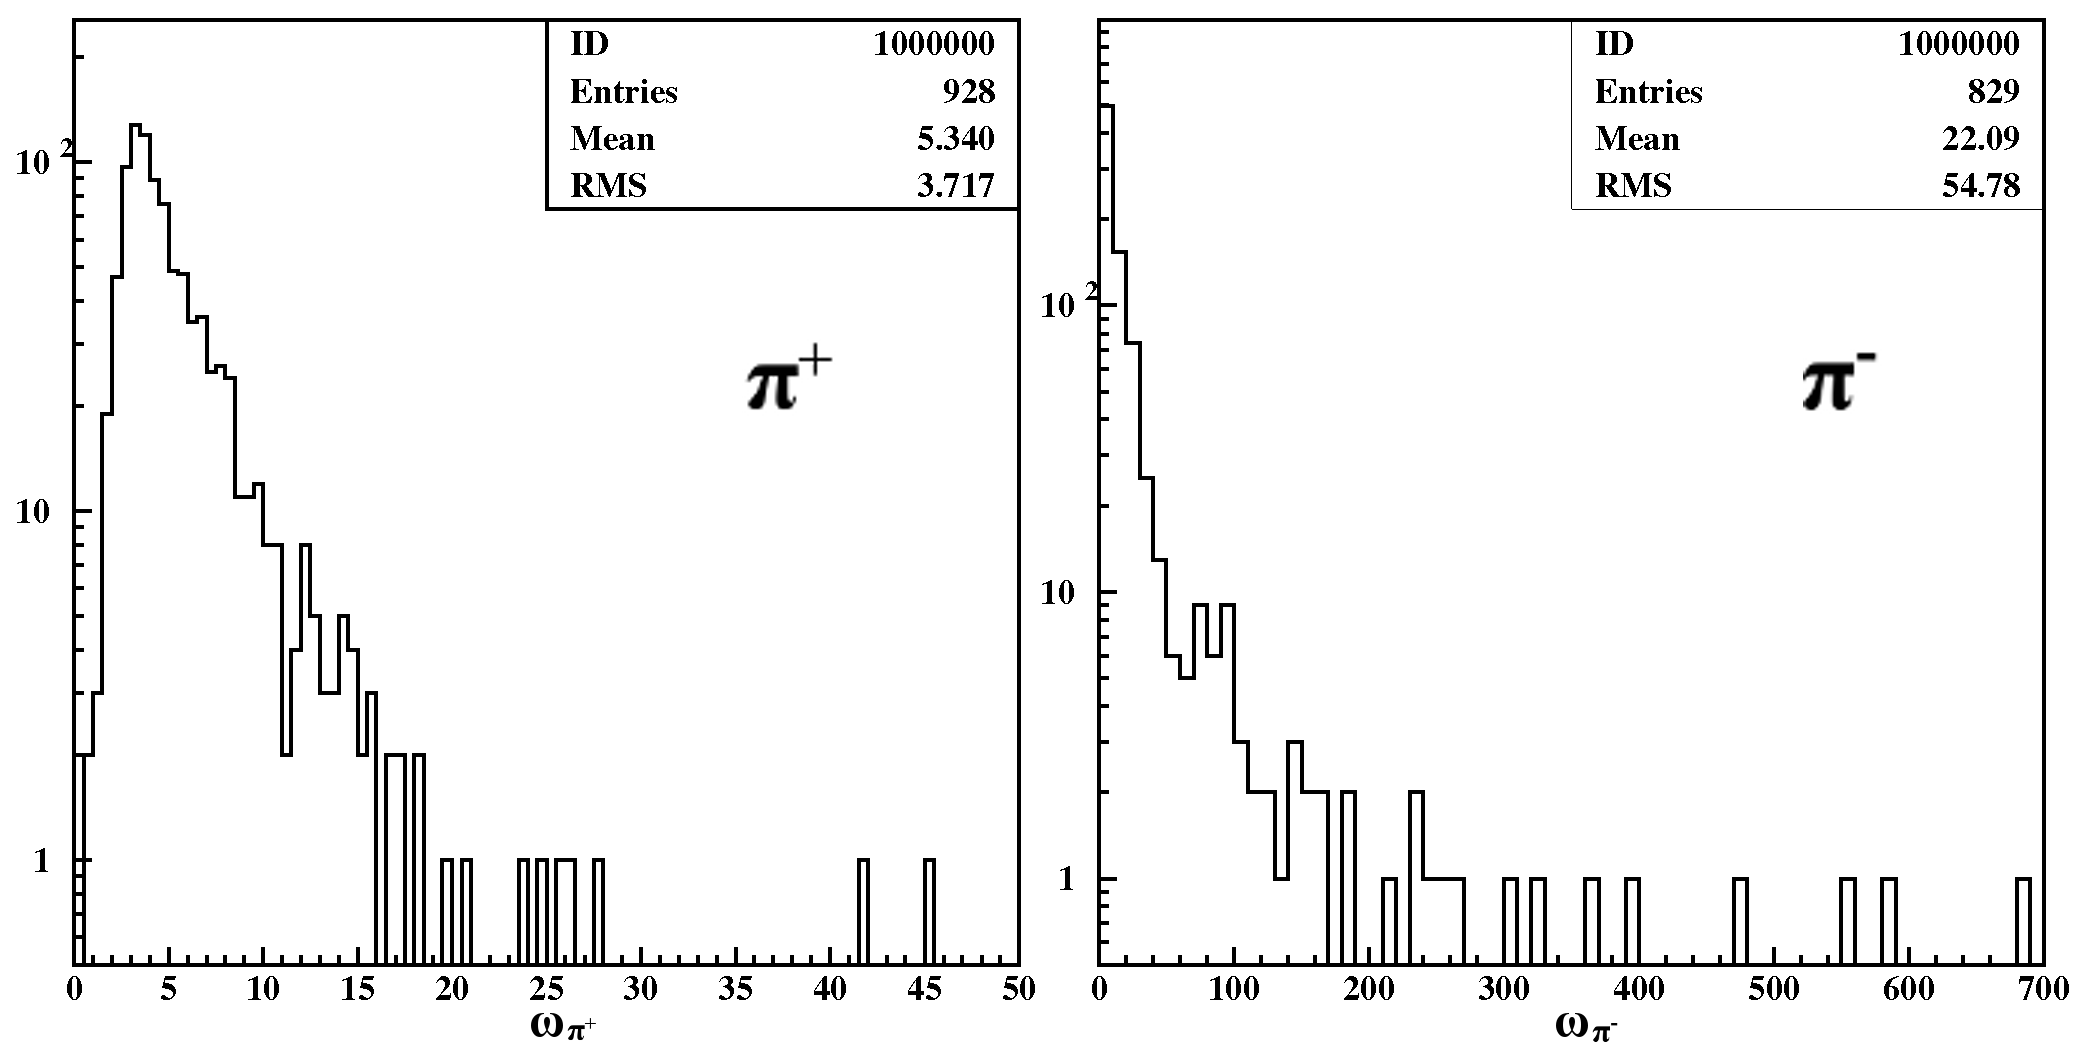
\includegraphics[width=14cm] {chap5-fig/pawpipdeut.png}
\caption {Acceptance weights for pions in deuterium (not reweighted).}
\label{fig:AccCoef}
\end{figure}

The electron acceptance, necessary in order to correct the number of electrons 
in the multiplicity ratios, is done with the same method than in the 
semi-inclusive case, but only using the two first dimensions ($\nu$ 
and $Q^2$). It is also interesting to note that no reweighting is necessary 
for electrons as all non-empty bins pass the cuts \ref{eq:AccL1} and 
\ref{eq:AccL2}.

\begin{figure}[tbp]
\centering
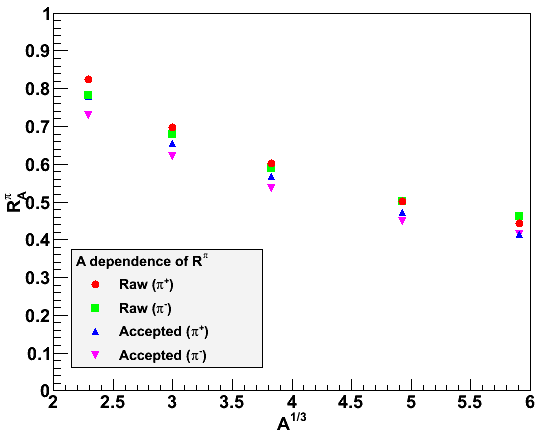
\includegraphics[width=7.4cm] {chap5-fig/b_RvA.png} 
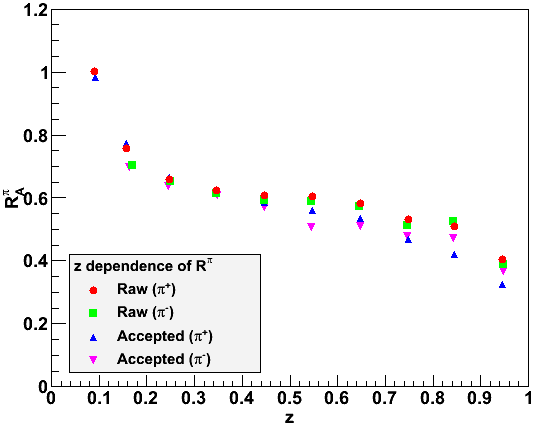
\includegraphics[width=7.4cm] {chap5-fig/b_RvZ.png} 
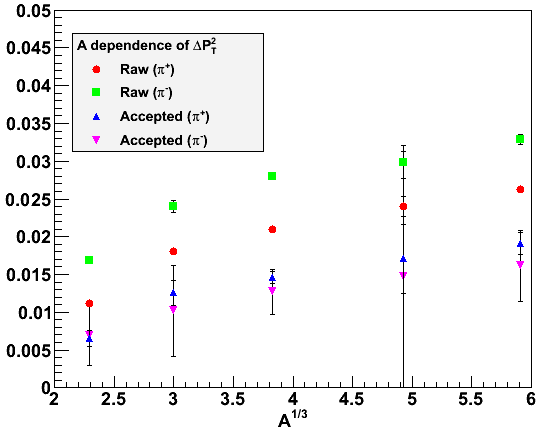
\includegraphics[width=7.4cm] {chap5-fig/b_PvA.png} 
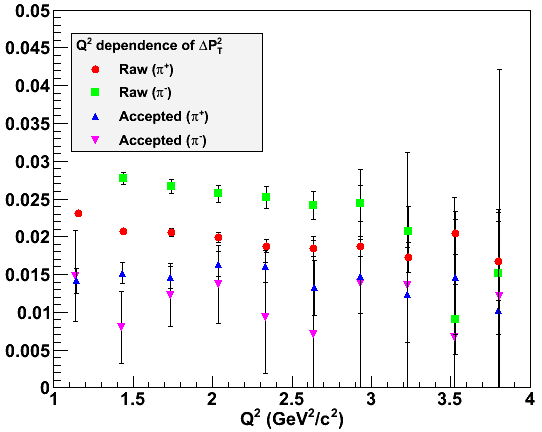
\includegraphics[width=7.4cm] {chap5-fig/b_PvQ2.png} 
\caption {Preliminary results are compared with results corrected for 
acceptance, for multiplicity ratios (top) and transverse momentum broadening 
(bottom). Only statistical errors are shown.}
\label{fig:AcceptPlots}
\end{figure}

Figure \ref{fig:AcceptPlots}, where only statistical errors are 
represented, shows the new results after applying the acceptance correction.
The acceptance effects appear to be of $\sim 10$\% for multiplicity ratios and 
$\sim 30$\% for transverse momentum broadening. This is a surprisingly 
significant correction for the few centimeters between the two targets. The 
$\pi^-$s are more affected because of CLAS' magnetic field. Indeed, the low \pt
$\pi^-$s have very low acceptance, this makes the errors 
on \dpt very large and the related results difficult to exploit. Finally, because 
of some difference in position between the solid targets (table 
\ref{tab:targets}), some extra simulation is needed in order to exploit 
correctly the aluminum and tin results. Therefore, these two targets should not be considered for 
the final results.

\subsubsection{Coulomb Correction}
\label{CCor}

The large charge of the nuclear targets create an electric field that should 
be accounted for at our energies. This nuclear electric field accelerate or 
decelerate the incoming and outgoing charged particles, it also has non 
trivial effects such as focussing effects at lower energies. Aste {\it et 
al.}~\cite{Aste:2005wc} have shown that an effective momentum approximation is 
reliable for larger momentums ($Q^2>.5$ GeV$^2$). Being clearly beyond this 
limit and the Coulomb correction being relatively small in our kinematic, we 
decide to use such an approximation. Following the prescription from Aste 
{\it et al.} we use an effective potential $\bar V= 0.8 V_0$, that they found 
best suited when using such approximation. $V_0$ being the electrostatic 
potential in the center of the nuclei, {\it i.e.}: $V_0= -3 \alpha_{EM} Z / 
(2 R)$. Values for $V_0$ and $\bar V$ used in this analysis are given in 
table~\ref{tab:Coulomb}. Coulomb corrections are applied on electrons, and
both charged pions before to calculate the kinematic variables.

\begin{table}[htbp]
  \centering
  \begin{tabular}{@{} ccc @{}}
    \hline
Nucleus & $V_0$ (MeV)  &  $\bar V$ (MeV) \\ \hline
$^2$H  & -1  &     -1 \\
C   &  -4 &      -3 \\
Al  &  -7 &      -6 \\
Fe  & -11 &    -9 \\
Sn  & -17 &   -14 \\
Pb  & -23 &   -19 \\
    \hline
  \end{tabular}
  \caption{Values for $V_0$ and $\bar V$ used for Coulomb correction of charged particles.}
  \label{tab:Coulomb}
\end{table}


\subsubsection{Radiative Correction}
\label{RadCor}

Despite its lower magnitude, compared to the strong force, the 
electromagnetic force might have a non negligible impact on our results. The 
reason is that even a moderate energy photon 
emission can modify significantly the measured kinematic variables.
To correct this effect, several simulation codes exist \cite{Akushevich:2001yp}, 
however, none permit to treat directly semi-inclusive DIS on nuclei. In order 
to make the correction, a dedicated Monte-Carlo simulation, based on existing 
codes, was developed.

\paragraph{Simulation}

The inclusive radiative effects are generated using the RADGEN software 
\cite{Akushevich:1998ft}, which includes the Feynman diagrams shown in 
figure~\ref{fig:FDRadCorr}. This code evaluates directly the correction 
factors ($\delta = \sigma_{obs} / \sigma_{Born}$) to apply for inclusive 
measurements. As RADGEN is also a Monte-Carlo generator of photon emissions, 
it can be used to modify the virtual photon kinematic before the 
hadron production in any DIS generator. This allows to evaluate the radiative 
effects on semi-inclusive measurements by implementing RADGEN inside a full 
Monte-Carlo event generator.

\begin{figure}[htbp]
\centering
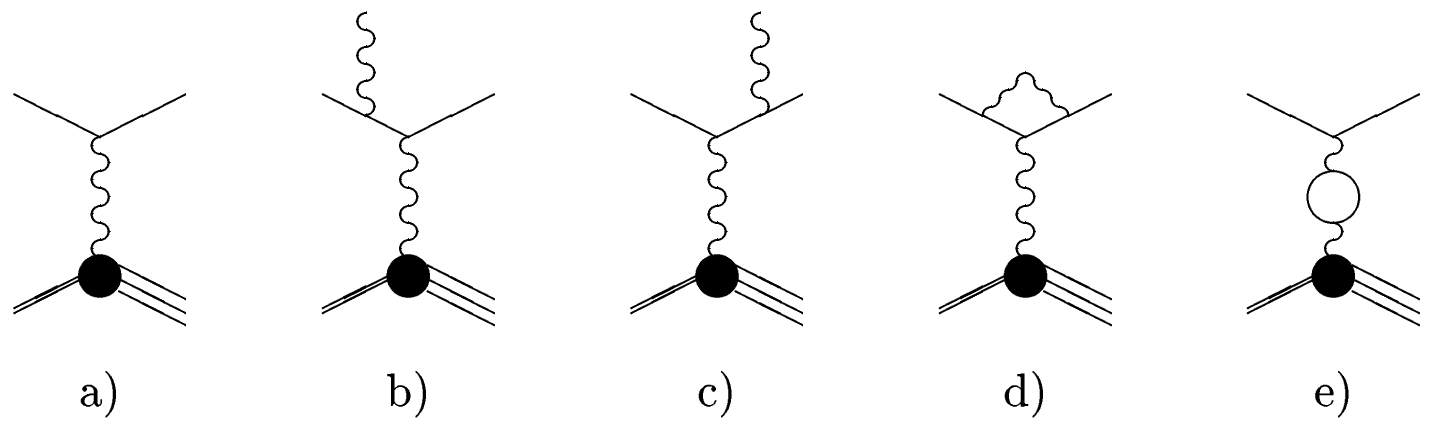
\includegraphics[width=12cm] {chap5-fig/RadDiag.png}
\caption {Diagrams taken into account in RADGEN \cite{Akushevich:1998ft}. The 
diagrams b) to e) contribute to the first order calculation of the radiative 
effects on Born cross section (diagram a)).}
\label{fig:FDRadCorr}
\end{figure}

The Monte-Carlo simulation we use is the GENIE software 
\cite{Andreopoulos:2009rq}, which describes well electron-nuclei scattering. 
Indeed, GENIE includes quasi-elastic scattering\footnote{Elastic 
scattering on a single nucleon of a nuclei.}, which is the main channel contributing 
to the radiative events in the DIS region \cite{Akushevich:2007jc}. The GENIE 
software includes also hadron cascades in the nuclei, which lead to the 
possibility to generate pions in quasi-elastic events. This is an important 
feature because the quasi-elastic cannot contribute directly to semi-inclusive 
measurements.

\paragraph{Correction of the Data}

We generate 100 million events per target, with and without radiative effects.
The RADGEN software gives direct indication for the inclusive correction and 
the comparison between the two data sets allows to extract factors for 
semi-inclusive correction.

The correction factors for inclusive ratio (figure \ref{fig:RadCorrFac}) are 
relatively small (couple of percents maximum) except at low \xb and high $\nu$. Semi-inclusive factors are 
shown in figure \ref{fig:RadCorrFacSIDIS} as a function of $z$ and \ptp. However 
the statistical error on these is large, the problem being that only a small 
fraction of the events involved photon radiation.

\begin{figure}[htbp]
\centering
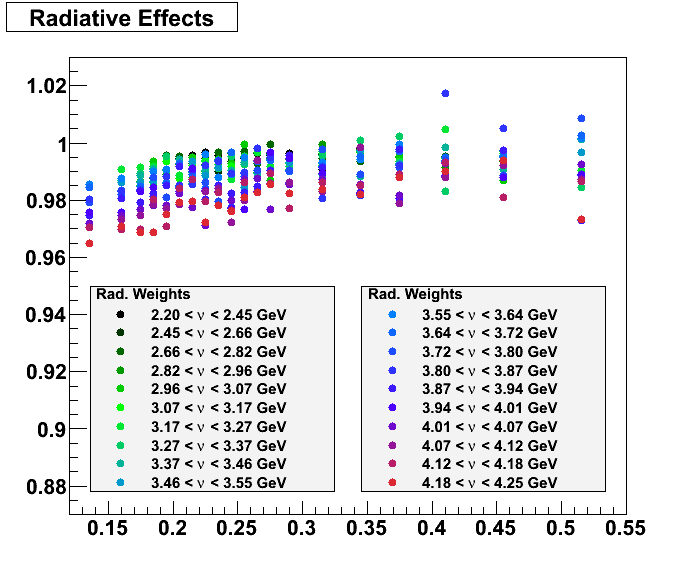
\includegraphics[width=9cm] {chap5-fig/ElecRadWei_Lead.png}
\caption {Ratios of the radiative correction factors $\delta_\text{Pb}/
\delta_{^2\text{H}}$ as a function of \xb in various $\nu$ bins.}
\label{fig:RadCorrFac}
\end{figure}

\begin{figure}[htbp]
\centering
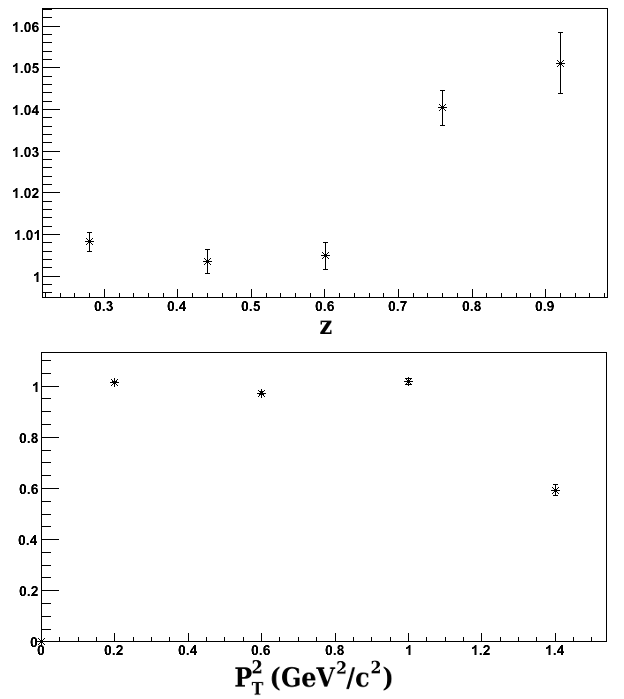
\includegraphics[width=9cm] {chap5-fig/RadGenFactors.png}
\caption {Ratios of the radiative correction factors $\delta_\text{Pb}/
\delta_{^2\text{H}}$ as a function of $z$ and \ptp.}
\label{fig:RadCorrFacSIDIS}
\end{figure}

The radiative correction appears to be limited in amplitude in most of the 
kinematic, so we decided not to apply it before further studies. Improvement can 
be easily obtained by generating more statistics, in order to analyze the 
semi-inclusive effects in more depth. Also radiative effects from the target thickness 
are ignored in the current setup; these need to be evaluated and, eventually, 
corrected as well.

\subsubsection{Isospin Correction}

The important excess of neutron in heavy nuclei leads to a modification of the 
$\pi$ multiplicity per DIS events. Using Hall~C results 
\cite{Asaturyan:2011mq}, shown in figure \ref{fig:IsoSpin}, we evaluate 
correction factors for this effect. Our simple estimation is solely based on 
proton and neutron numbers; the results for $\pi^+$s are shown in 
table~\ref{tab:isospin}. The effect on $\pi^-$ is found to be coherent with zero,
therefore no correction is applied for them. 
We attribute errors of 10\% of the effect for the isospin correction, this is chosen 
relatively to the precision of the Hall~C measurement.

\begin{figure}[tbp]
\centering
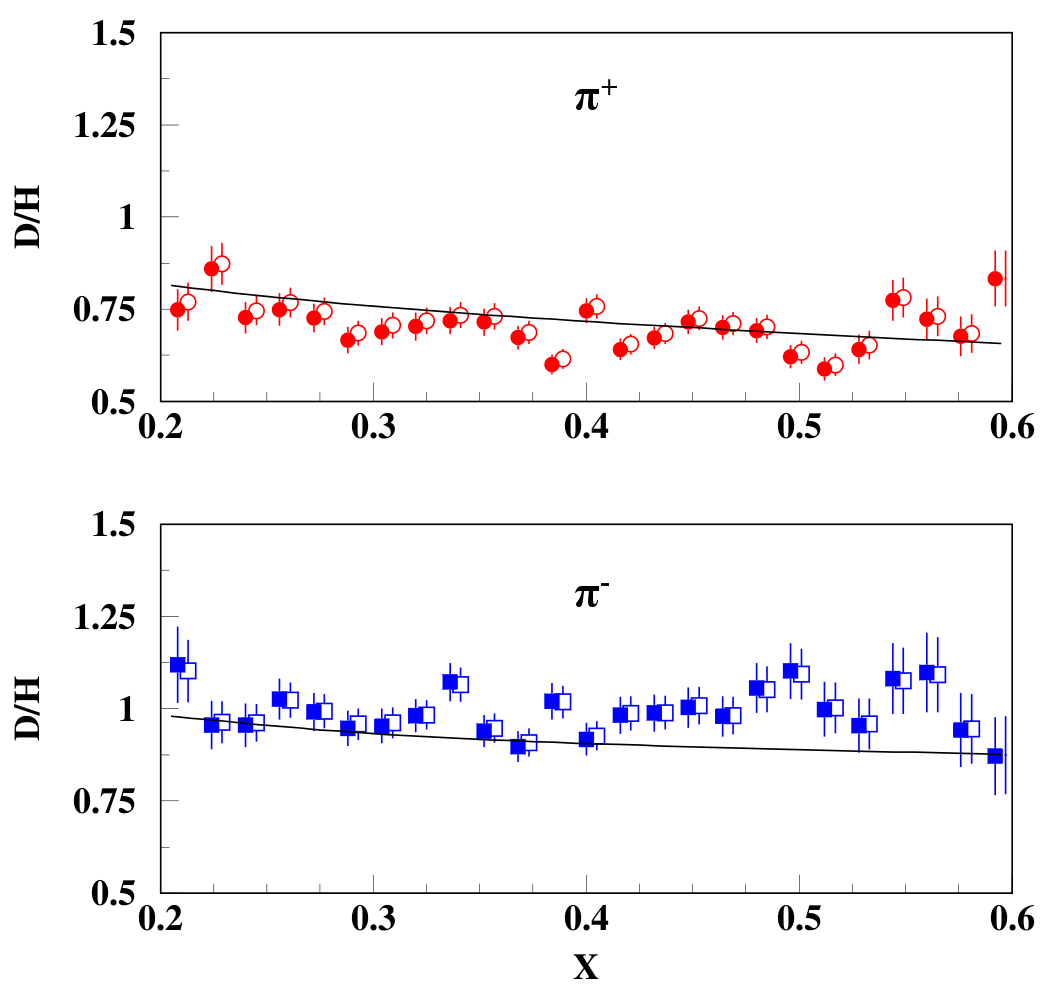
\includegraphics[width=10cm] {chap5-fig/HallC-Isospin.png}
\caption {Ratios of deuteron over proton for $\pi^+$s and $\pi^-$s 
as a function of \xb at $z=0.55$ \cite{Asaturyan:2011mq}.}
\label{fig:IsoSpin}
\end{figure}

\begin{table}[htbp]
  \centering
  \begin{tabular}{@{} cc @{}}
    \hline
    Target & Isospin  \\ 
           & correction \\ 
    \hline
    C & 0 \\
    Al & 1.5\%\\
    Fe &  3\% \\
    Sn &  8\%\\
    Pb &  10\% \\
    \hline
  \end{tabular}
  \caption{Isospin correction applied to the $\pi^+$ multiplicity ratios for different targets.}
  \label{tab:isospin}
\end{table}

It is important to note that we correct isospin effects only for rates, thus 
we correct only the multiplicity ratios. Transverse momentum broadening could, in 
principle, also be affected, however, the results from \cite{Asaturyan:2011mq} 
show no isospin effect in \ptp. This gives good confidence that \dpt is not 
affected by isospin effects.

We finally note that the $A$ dependencies of the multiplicity ratios of the 
charged pions are similar after the isospin correction\footnote{Within 
normalization errors presented in section \ref{sec:TotSys}} (figure 
\ref{fig:IsoPlot}). Considering previous measurements and existing models, 
this result was expected and confirm the need for this correction to be applied.

\begin{figure}[tbp]
\centering
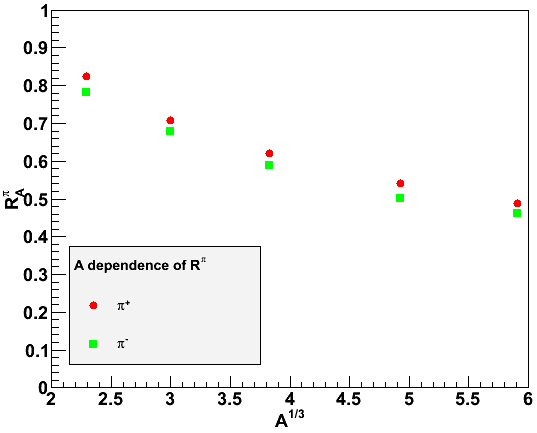
\includegraphics[width=8cm] {chap5-fig/c_RvA.png}
\caption {Multiplicity ratios as a function of $A^{1/3}$ 
with only isospin correction applied.}
\label{fig:IsoPlot}
\end{figure}

\subsection{Systematic Uncertainties}
\label{sec:TotSys}

In this section are summarized the systematic errors that we identified. The 
systematic point to point errors are calculated bin by bin for each results.
They are caused by uncertainties on the acceptance and on the identification of 
particles. The normalization errors are attributed globally. They are due to 
acceptance effects, target misidentifications and isospin correction.

\subsubsection{Quality of the Detection}
\label{SysId}

The simulation of the CLAS detector, using GSIM package, is used 
to evaluate the systematic errors linked with:

  - experimental resolution of kinematic variables,

  - particle misidentification,

  - particle re-scattering in the detector,

  - particle energy loss.\\


To evaluate those errors, we compare the reconstructed particles with the 
generated ones. Each reconstructed particle is associated with its generated parent using the
similarity in momentum and angle.
Distributions of $\Delta p$, $\Delta \theta$ and $\Delta \phi$ are defined as 
$\Delta x = {\sum_n |x_{gen} - x_{rec}| \over n}$. They give the precision with which we measure 
these variables. Using the same simulation than for the acceptance, we find 
${\delta p \over p } = 0.03$, $\delta \theta = 3$ mrad and 
$\delta \phi = 10$~mrad. These are broader than announced in \cite{Mecking:2003zu} 
but still reasonable. Then associated systematic errors can be easily 
evaluated for other variables: $\delta Q^2 \sim 0.013$ GeV$^2$/c$^2$, $\delta z \sim 
0.4 \%$, $\delta P_\perp^2 \sim 0.004$ GeV$^2$/c$^2$ and so on\footnote{These were 
evaluated for typical kinematics, the results can be significantly larger at 
extreme kinematics (large \pt or Q$^2$).}. These are negligible because they are 
several times smaller than our usual bin sizes (see figures in section 
\ref{prelim}). 

We also evaluate particle misidentification and particles originating from 
scattering in the detector or the coils. Only tails of distributions can lead to high 
contamination by misidentification, the most problematic being the tail of the 
\pt distribution. This effect is due to the low probability to produce high 
\pt events, therefore the contribution from accidental is relatively 
increased. We use the following cut $p_\perp^2 < 2.5$~GeV$^2$/c$^2$, which 
only removes a very little amount of data ($\sim 1$ $\pi$ in 30000). The 
misidentification of electrons is found to be of the order of 1 in a 1000 and 
does not contribute significantly to the uncertainty. For pions, the main 
contamination comes from kaons above 2~GeV/c ($\sim$3\% of $\pi^+$ and 
$\sim$0.5\% of $\pi^-$). Incidentally, protons also contaminates $\pi^+$ at 
high momentum (up to few \%). The uncertainty related to 
misidentification is taken into account for the point to point systematic error 
evaluation, other effects are found to be negligible.

\subsubsection{Target Reconstruction}

Because of reconstruction errors or scattering on the detector materials, it 
is possible to associate a particle with the wrong target. To estimate this 
effect, we look, in the experimental data, at the number of events 
reconstructed upstream and downstream of the targets, where nothing should be
detected. We define two test regions (see figure \ref{fig:targetleak}) to evaluate
the contamination. The region 1 is upstream and chosen to be of the same size as the window used for solid 
target selection. We use it to evaluate contamination from the liquid target to the solid one. The region 2
is downstream and of the size of the window for the liquid target selection and allows to evaluate the solid target leak into the liquid one
The distance between detection and test regions is identical to the 
distance between the two detection regions. 

We find
that the number of electrons in the test regions 1 and 2 represent 1 and 2\%, 
respectively, of the total number of events. In the case of semi-inclusive measurement, where we request
2 particles in the final state, the number drops drastically and is of the order of
0.01\%. In conclusion, only the number of electron is significantly affected by this problem
leading to a normalization error of 1\% for all multiplicity ratios.

\begin{figure}[tbp]
\centering
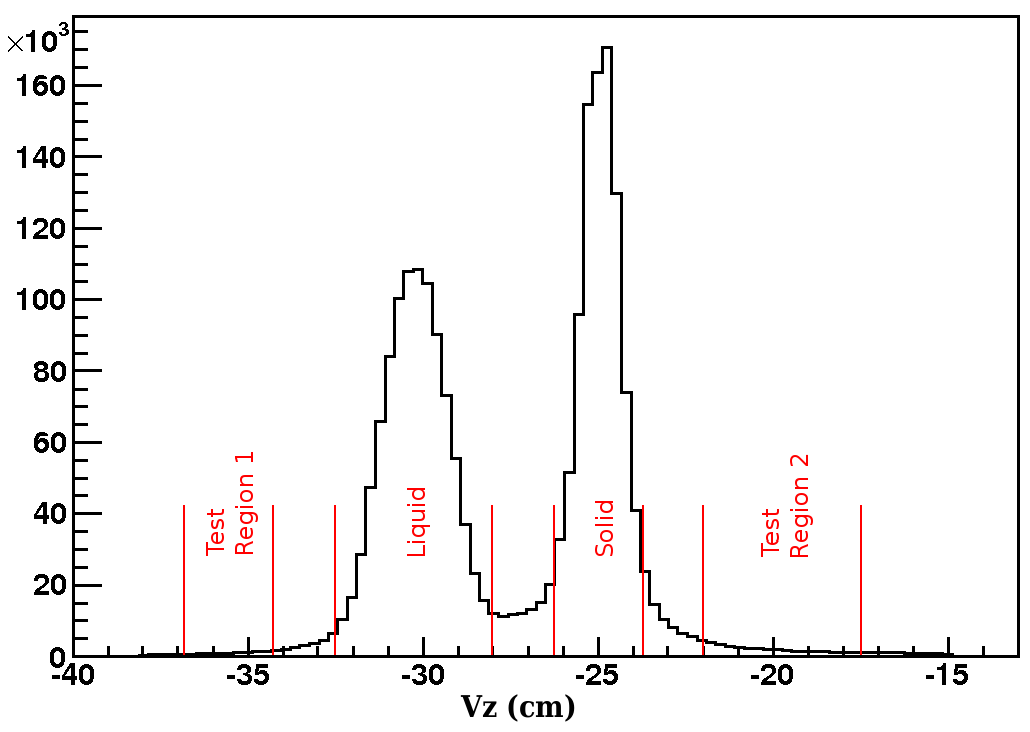
\includegraphics[width=9cm] {chap5-fig/Vertex.png}
\caption {Distribution of the vertex positions along z (cm), i.e. along the 
beam line. In red are shown the cuts used to evaluate the leak from one target to 
another.}
\label{fig:targetleak}
\end{figure}

\subsubsection{Acceptance}

We apply two different acceptance corrections to the data using two different binnings 
(table \ref{tab:AcceptBinning}). The differences between them give us a good 
indication on the systematic error associated with the method. Using a sample 
of results from iron, we find the systematic presented in the table 
\ref{tab:SysAcc}. We note the significantly larger errors for $\pi^-$, which 
was expected because of the smaller acceptance and the larger weights. More 
significant are the large errors on the \dpt measurements, this is mainly due to 
the nature of the observable; as a difference \dpt enhances relative errors 
significantly. As was seen in figure~\ref{fig:AcceptPlots}, error bars are much 
larger for corrected \dpt indicating an important statistical 
sensitivity introduced by the weighting. The errors on \dpt are of the same 
order, or smaller, as the differences observed between the two sets. This is 
an indication that the uncertainties reported in table \ref{tab:SysAcc} are already 
taken into account in the statistical error.

\begin{table}[htbp]
  \centering
\renewcommand{\arraystretch}{1.3}
  \begin{tabular}{|c|c|c|}
    \hline
    Variable & Normalization & Point to point \\ 
             & errors        & errors         \\ 
    \hline
    $R^{\pi^+}_A$  & 1.2\% & 1.5\%  \\
    $R^{\pi^-}_A$  & 2.5\% & 2.6\%   \\
    $\langle \Delta P_\perp^2 \rangle^{\pi^+}_A$ & 5\% & 11\% \\
    $\langle \Delta P_\perp^2 \rangle^{\pi^-}_A$ & 5\% & 21\% \\
    \hline
  \end{tabular}
  \caption{Relative errors on observables between the two weighting 
  described in the text.}
  \label{tab:SysAcc}
\end{table}

\subsubsection{Normalization Error}

The normalization errors -- i.e. independent of kinematic variables -- are due to acceptance effects, target identification 
and isospin correction. They are summarized in the table \ref{tab:sysid}. 

\begin{table}[htbp]
  \centering
\renewcommand{\arraystretch}{1.3}
  \begin{tabular}{|c|cc|cc|}
    \hline
              & $R_A^{\pi^+}$  & $R_A^{\pi^-}$ & \dptp$^{\pi^+}$ &  \dptp$^{\pi^-}$\\ 
    \hline
    Acceptance & 1.2\% & 2.5\% & 5\% & 5\% \\
    Target id. & 1\% & 1\% & 1\% & 1\% \\
    Isospin (Pb)& 1\% & 1\% & 1\% & 1\% \\
    Total      & 1.9\% & 2.9\% & 5.2\% & 5.2\% \\
    \hline
  \end{tabular}
  \caption{Normalization uncertainties.}
  \label{tab:sysid}
\end{table}



\section{Results and Discussions}
\label{chap:results}

The results presented in this chapter are a selection of the observables 
that we want to use in the first publication, eventually a long paper will
include results as function of all variables. All results were extracted with the following DIS selection cuts: 
$Q^2$~$>$~$1$~GeV$^2$/c$^2$, $W$~$>$~$2$ GeV and $y<0.85$. To ensure that SIDIS 
factorization applies~\cite{Mulders:2000jt}, we are selecting events with 
$0.4$~$<$~$z$~$<$~$0.7$~\footnote{This cut is not applied for plots with results 
as a function of $z$.} based on the previously published results from 
\cite{Asaturyan:2011mq}. Moreover, this cut also ensures that we are measuring the 
leading hadron, and avoiding the high $z$ region, which might be contaminated by 
the decay products of the diffractive production of $\rho^0$. Finally, we are 
applying a cut on $x_F > 0$ to select the forward fragmentation region.

\subsection{Multiplicity Ratio}

\subsubsection{$A$ Dependence}
\label{sec:resA}

\begin{figure}[p]
\centering
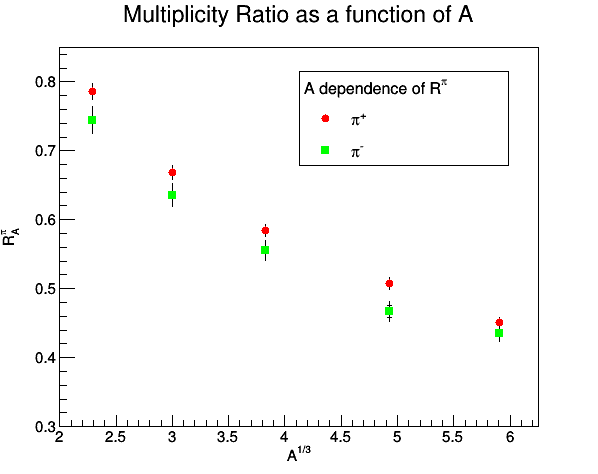
\includegraphics[width=7.4cm] {chap6-fig/F_RvA.png} 
\caption {$A^{1/3}$ dependence of the multiplicity ratio. Normalization 
uncertainties are not shown.}
\label{fig:RA}
\end{figure}

Figure \ref{fig:RA} contains our results for the $A^{1/3}$ dependence of 
the multiplicity ratio. One can see a 5\% normalization difference between both pions. However, this difference is not significant as it represents only 1.5 
standard deviation of our normalization uncertainty (see table~\ref{tab:sysid}).

The attenuation, presented in the figure \ref{fig:RA}, is neither linear as a 
function of $A^{1/3}$ nor as a function of $A^{2/3}$. The HERMES data had
already showed some indication 
of this feature~\cite{Airapetian:2007vu,Airapetian:2009jy}, but here the 
non-linearity, which has important implication on models, is clear. Indeed, 
it seems difficult to reconcile the prehadron absorption models with this result. Prehadrons 
are expected to have their cross sections increasing with time and, therefore, 
distance. On the parton energy loss side, the BDMPS calculation gives a parton 
energy loss proportional to $L^2 \propto A^{2/3}$, indicating that we are not
in the region where this result applies. Morover, if the production 
time\footnote{As defined in figure~\ref{fig:hadro}} occurs 
inside the nuclei, the behavior of the multiplicity ratio can be more complicated
as different processes intervene.

\subsubsection{Cronin Effect}

\begin{figure}[p]
\centering
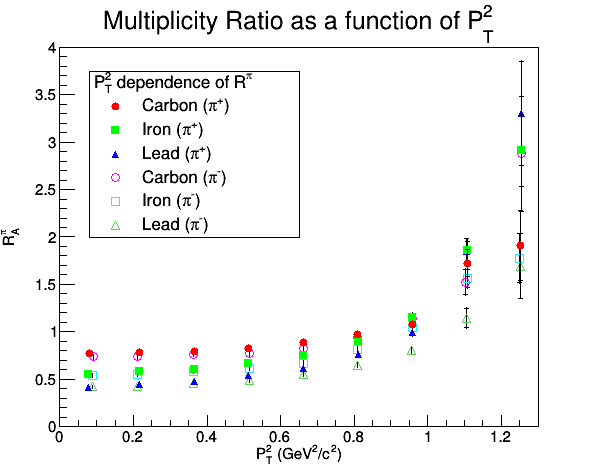
\includegraphics[width=7.4cm] {chap6-fig/F_RvPt.png} 
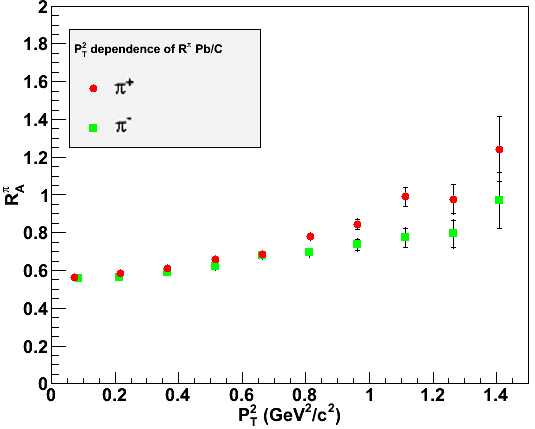
\includegraphics[width=7.4cm] {chap6-fig/F_RvPt_PbC.png} 
\caption {Multiplicity ratios as a function of \pt (GeV$^2$/c$^2$) for both charged pions. Left: The usual multiplicity ratio results. Right: Lead results normalized to carbon. Normalization uncertainties are not shown.}
\label{fig:RPt}
\end{figure}

\begin{figure}[p]
\centering
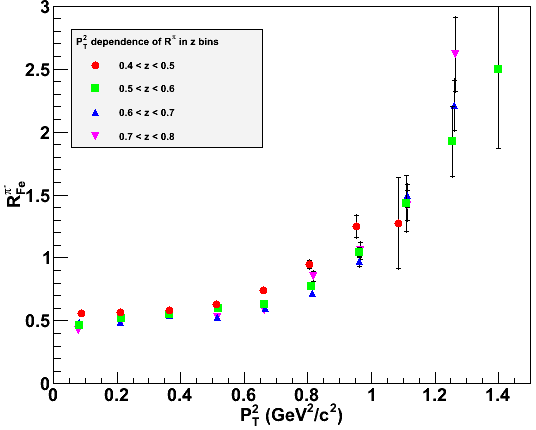
\includegraphics[width=7.4cm] {chap6-fig/F_RvPtinZ.png} 
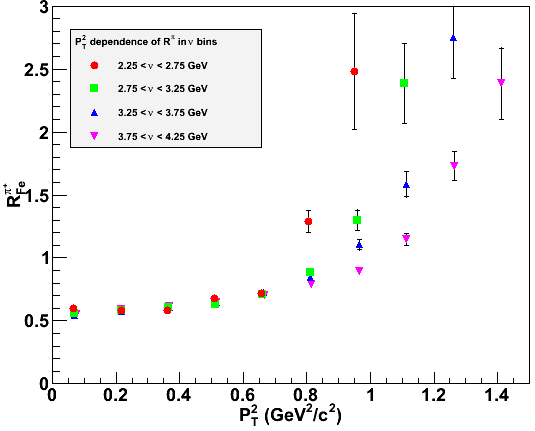
\includegraphics[width=7.4cm] {chap6-fig/F_RvPtinNu.png} 
\caption {Positive pions multiplicity ratios as a function of \pt (GeV$^2$/c$^2$) for different $z$ bins (left), and different $\nu$ (GeV) bins (right). Normalization uncertainties are not shown.}
\label{fig:RPtMulti}
\end{figure}

The Cronin effect is characterized by a large increase of the multiplicity 
ratio at high \pt ($\sim$1~GeV$^2$/c$^2$), which is a controversial result in hadronization studies. Indeed, whereas SLAC measurements 
\cite{Osborne:1978ai} did not show such an effect, HERMES \cite{Airapetian:2007vu} measured a significant increase of the multiplicity 
ratio with \ptp. Our result (figure \ref{fig:RPt} (left)), integrated over 
all other variables, showed a pattern similar to the HERMES measurement. 
However, there are some potential contributions from the target fragmentation and 
the Fermi motion.

Fermi motion effects can be significantly reduced by modifying our regular observables. Indeed, using carbon for normalization, instead of deuterium, most effects of Fermi motion cancel out. Moreover, acceptance effects (section~\ref{sec:accept}) will also be mostly canceled in such a ratio, leading to a reduction of their systematic errors dominated mainly by the normalization error. The normalized lead multiplicity ratio to carbon is presented on figure \ref{fig:RPt} (right). There is an attenuation, at low \ptp, similar to the usual multiplicity ratio of iron. This can be understood based on the difference of both nuclei radii, $R_{Pb}-R_{C} \sim R_{Fe}$. Nevertheless, the observed enhancement with \pt is much more modest than in iron. At first sight the difference can be attributed to Fermi motion, which might affect the normalized measurement with deuterium compared to carbon.

In figure \ref{fig:RPtMulti}, the multi-dimensional multiplicity ratio results are presented. HERMES found an important $z$ dependence of the Cronin effect \cite{Airapetian:2007vu,Airapetian:2011jp}. That can be treated as a sign of an essential contribution from a target fragmentation. The present result 
(figure~\ref{fig:RPtMulti} (left)) does not show this behavior, which could be due to our strict cut on $z$ ($z>0.4$ whereas HERMES used $z>0.2$) that leads to a smaller target fragmentation contamination. The second result, binned in \pt and $\nu$ (figure \ref{fig:RPtMulti} (right)), showed an important 
$\nu$ dependence of the Cronin effect. However, HERMES results did not exhibit such a $\nu$ behavior. This is a clear evidence of the importance of 
the Fermi motion effect in our measurement.

The result of the lead to carbon multiplicity ratio, figure \ref{fig:RPt} 
(right), has another interesting feature: the $\pi^+$s have a stronger Cronin 
effect. However, the significance of this observation is not clear. This could be 
a contribution from target fragmentation, as we might expect more positive 
particles would originate from nuclei than negative ones. This could also come from other sources such as the isospin effect or a factorization breaking at high 
\ptp. However, no test of these features exists in our kinematical range\footnote{Results of \cite{Asaturyan:2011mq} covered only \pt$<0.2$ GeV$^2$/c$^2$.}. Last but not least, it could be correlated with the hadronic rank and reflect some hadronization properties. Indeed, as we probe mostly valence quarks at our energies, $\pi^+$s are more likely to be the leading hadrons compared to $\pi^-$s.

In conclusion, our results indicate that the HERMES results were affected by a target fragmentation and that our results are affected by the Fermi motion. These effects can be easily controlled by a careful selection of our observables. In this regard, the Pb/C ratio seems to give cleaner results than Fe/D.

\subsubsection{$\nu$ Dependence}

\begin{figure}[tbp]
\centering
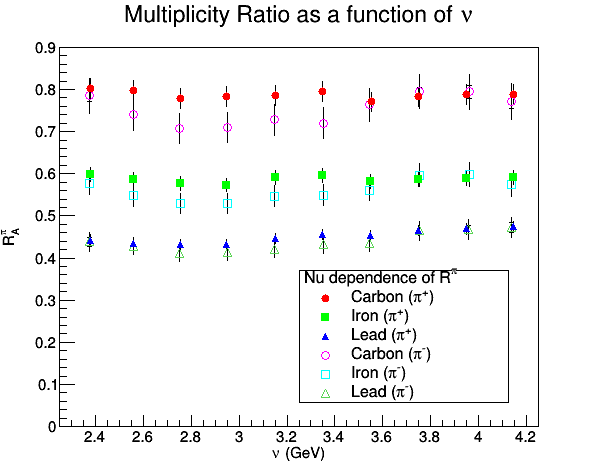
\includegraphics[width=7.4cm] {chap6-fig/F_RvNu.png} 
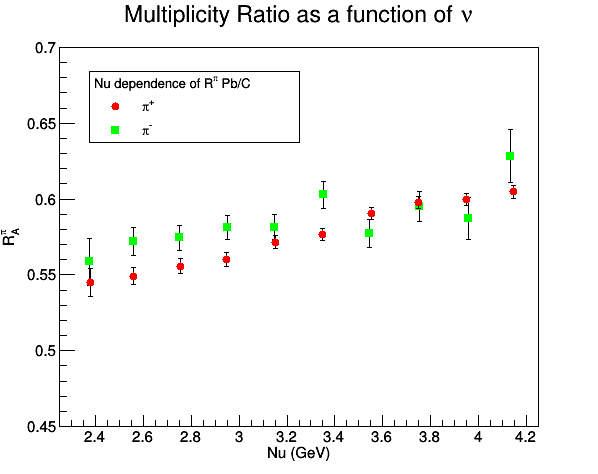
\includegraphics[width=7.4cm] {chap6-fig/F_RvNu_PbC.png} 
\caption{Multiplicity ratios as a function of $\nu$ (GeV) for both charged pions. Left: The usual multiplicity ratio results. Right: Lead results normalized to carbon. Normalization uncertainties are not shown.}
\label{fig:RNu}
\end{figure}

The HERMES collaboration clearly observed a rise of the multiplicity ratio 
with $\nu$ from 6 to 22~GeV. However, our results (figure \ref{fig:RNu} (left))
show no dependence, besides a slight increase in lead.
However, the Fermi motion could cancel most of this hadronization effect, and 
what is left will be washed out with the acceptance correction systematic 
uncertainty. The normalized multiplicity ratio to carbon offers a 
cleaner result, that is not affected by Fermi motion or acceptance. For this
observable, we measure a slope consistent with what was observed by HERMES.

We must note the similar behavior of both pions results in a figure 
\ref{fig:RNu} (right). This confirms our previous remark that the difference 
observed in the regular multiplicity ratio might originate from the 
normalization uncertainty caused by the acceptance correction. Also, there is no 
clear difference between both charged pions on the integrated multiplicity 
ratios as a function of $\nu$.

\subsubsection{$z$ Dependence}

\begin{figure}[tbp]
\centering
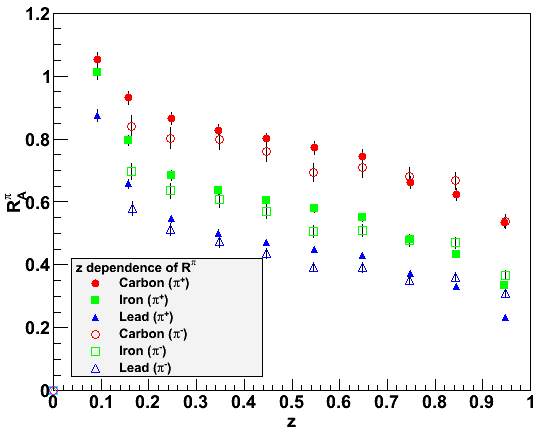
\includegraphics[width=7.4cm] {chap6-fig/F_RvZ.png} 
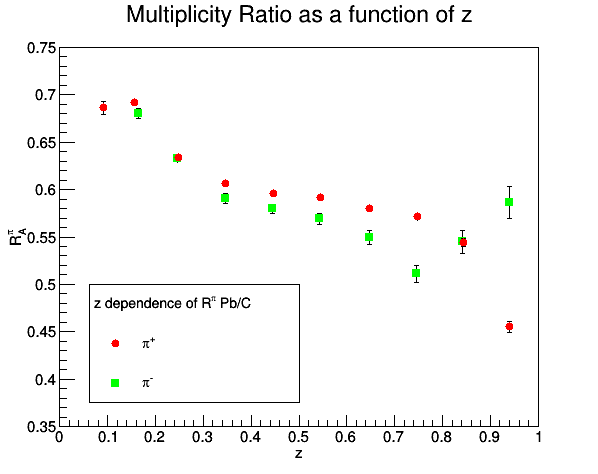
\includegraphics[width=7.4cm] {chap6-fig/F_RvZ_PbC.png} 
\caption {Multiplicity ratios as a function of $z$ for both charged pions. Left: The usual multiplicity ratio results. Right: Lead results normalized to carbon. 
Normalization uncertainties are not shown.}
\label{fig:Rz}
\end{figure}

The multiplicity ratio was observed to decrease with $z$ in HERMES data, 
whereas this behavior was not significant in other experiments. Indeed the 
nature of this behavior is questionable as the target fragmentation also get reduced 
with $z$, hence can mimic the signal. In figure \ref{fig:Rz} (left), as for HERMES results, we see a clear slope even at values higher than 0.4, where target fragmentation effects are expected to be small. However, the lead to carbon ratio (figure \ref{fig:Rz} (right)) shows a much flatter behavior in the region of interest (from 0.4 to 0.7). Therefore, this situation seems similar to the Cronin effect, where HERMES observation was enhanced by a target fragmentation. The measurement using the carbon as a basis is, therefore, more useful on isolating effects from the hadronization. However, the low $z$ behavior remains driven by the target fragmentation region. Another strange feature of the data is the behavior at higher $z$ (figure \ref{fig:Rz} (right)), where the two pions behave differently. However, there is a lack of solid theoretical grounds in this region to interpret this result.

\subsubsection{$Q^2$ Dependence}

The behavior of hadronization as a function of $Q^2$ is an important issue, that 
has direct implications on our understanding of nuclear matter properties in 
QCD. HERMES results, which covered $1<Q^2<10$~GeV$^2$/c$^2$, gave a hint of an 
increase of the multiplicity ratio with $Q^2$. Our result, in figure 
\ref{fig:RQ2}, does not indicate any $Q^2$ dependence, hence our 
conclusion is that the multiplicity ratio has no significant $Q^2$ dependence.

\begin{figure}[tbp]
\centering
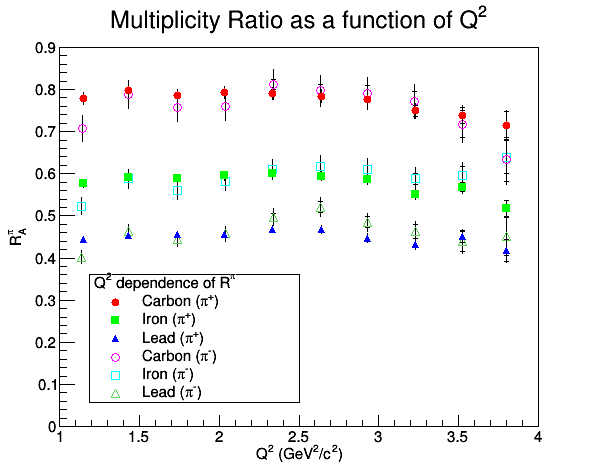
\includegraphics[width=7.4cm] {chap6-fig/F_RvQ2.png} 
\caption {Multiplicity ratios as a function of $Q^2$ (GeV$^2$/c$^2$). 
Normalization uncertainties are not shown.}
\label{fig:RQ2}
\end{figure}

We can use our large statistics to extract more information by handling the results differently. As a $\nu$ dependence is expected for the multiplicity ratio, it might be helpful to use a tighter $\nu$ bin to plot the $Q^2$ dependence (figure \ref{fig:RQ2Detailed} (left)), thus remove any coupling between the two variables.
As some Fermi motion effects would persist, it is more convenient to show the $Q^2$ dependence of the normalized multiplicity ratio of lead to carbon, see figure \ref{fig:RQ2Detailed} (right). The two results of figure \ref{fig:RQ2Detailed} 
showed a slight increase with $Q^2$, but as for HERMES, no evidence is 
reached on this context. Our leverage on $Q^2$ appears to be too modest to make a clear measurement. 

\begin{figure}[tbp]
\centering
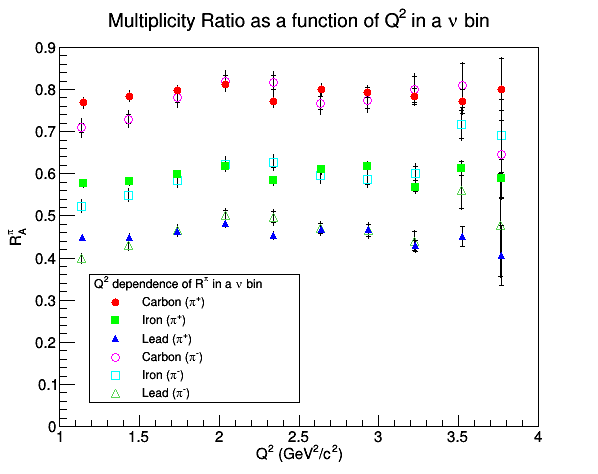
\includegraphics[width=7.4cm] {chap6-fig/F_RvQ2inNu.png} 
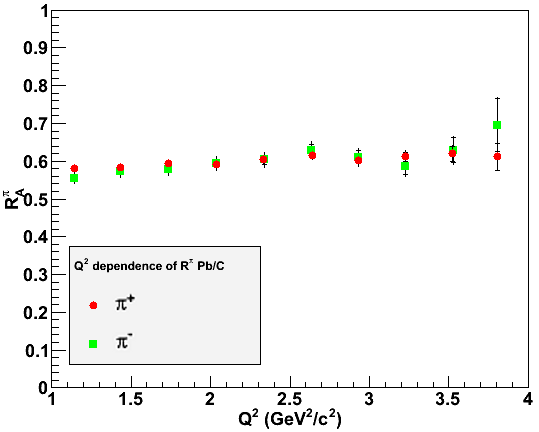
\includegraphics[width=7.4cm] {chap6-fig/F_RvQ2_PbC.png} 
\caption {Multiplicity ratios as a function of $Q^2$ (GeV$^2$/c$^2$) for both charged pions. Left: The multiplicity ratio for a tighter $\nu$ bin ($3.25 < \nu < 3.75$ GeV). Right: The normalized multiplicity ratio of lead to carbon. Normalization uncertainties are not shown.}
\label{fig:RQ2Detailed}
\end{figure}

\subsection{Transverse Momentum Broadening}

\subsubsection{$A$ Dependence}

The $A$ dependence of the transverse momentum broadening, presented in 
figure~\ref{fig:PA}, is a crucial result. The combination of our large 
statistics with a wide $A$ coverage gives an outright indication of $A^{1/3}$ 
dependence of \dpt. This \dpt effect is found to be much smaller than that seen 
by HERMES\cite{Airapetian:2009jy}, which is consistent with
 theoretical models predicting larger effects at larger energies. However, 
calculations of the parton energy loss from BDMPS \cite{Baier:1996sk} 
correlated \pt with the square of the nuclear radius. A feature that is not 
observed in our result. Although, by looking to the low energy of our CLAS 
experiment, one might argue the validity of a direct comparison with BDMPS 
calculations. Nonetheless, this result shows an unexpected pattern that 
remains to be explained. One possible interpretation is the occurrence of 
the production time inside the nuclei, as we proposed for the $A^{1/3}$ 
dependence of multiplicity ratios. In this case, the colored parton does 
not interact with the whole nucleus which limits the nuclear effect.

\begin{figure}[tbp]
\centering
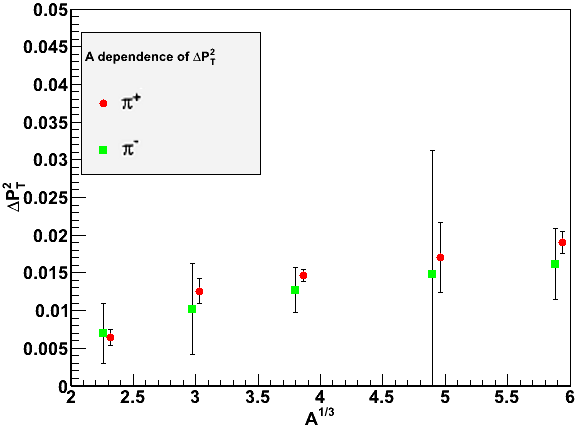
\includegraphics[width=8.2cm] {chap6-fig/F_PvA.png} 
\caption {$A$ dependence of \dptp. Points are slightly shifted for a readability. Normalization uncertainties are not shown.}
\label{fig:PA}
\end{figure}

\subsubsection{$Q^2$ Dependence}

Finally, the $Q^2$ dependence of \dpt is an important result for the BDMPS based 
calculation from \cite{Domdey:2008aq}. They predict a raise of \dpt with $Q^2$, 
which is not observed in figure \ref{fig:PQ2}. Using a tighter $\nu$ bin and a 
carbon normalization should isolate this effect better, but figure \ref{fig:PQ2-detailed}
gives a similar result. In conclusion, within error bars, no effect is observed for 
\dpt as a function of $Q^2$. However, we would like to have a quantitative theoretical 
input here, as it is not clear if we have the needed resolution to observe the effect 
expected within BDMPS based models. We are going to work with the authors of the original 
paper to add some projections on our figures.

\begin{figure}[tbp]
\centering
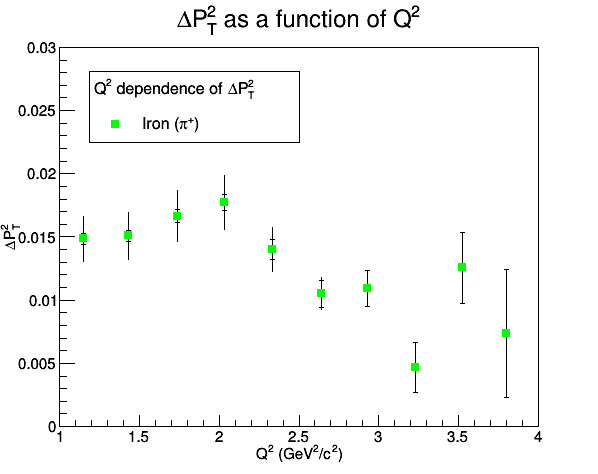
\includegraphics[width=7.4cm] {chap6-fig/F_PvQ2.png} 
\caption {Iron \dpt as a function of $Q^2$ (GeV$^2$/c$^2$) after applying the regular DIS cuts. Normalization uncertainties are not shown.}
\label{fig:PQ2}
\end{figure}

\begin{figure}[tbp]
\centering
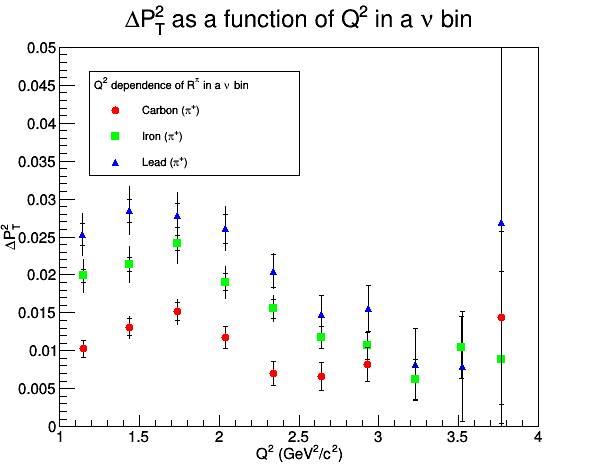
\includegraphics[width=7.4cm] {chap6-fig/F_PvQ2inNu.png} 
\includegraphics[width=7.4cm] {chap6-fig/F_PvQ2_PbC.png} 
\caption {Positive pions \dpt as a function of $Q^2$ (GeV$^2$/c$^2$). Left: The usual observable for a tighter $\nu$ bin ($3.25 < \nu < 3.75$~GeV). Right: \dpt 
of lead relative to carbon. Normalization uncertainties are not shown.}
\label{fig:PQ2-detailed}
\end{figure}



\bibliography{hadro}
\bibliographystyle{plain}

\end{document}
